\documentclass{article}
\usepackage{amsmath}
\usepackage{booktabs}
\usepackage{graphicx}
\usepackage{float}
\usepackage{hyperref}
\usepackage{multirow}
\usepackage{subcaption}
\usepackage{flafter}

\title{Homework 2}
\author{Zitian Wang}
\date{\today}

\begin{document}
\maketitle

\section{Exercise 1: Fourier Differentiation Matrix}

\subsection{Implementation of Odd Method}
The odd method for Fourier differentiation matrix is implemented with the following formula:
\begin{equation}
D_{ij} = \frac{(-1)^{i+j}}{2}\tan\left(\frac{(i-j)\pi}{N}\right), \quad i \neq j
\end{equation}
where $N$ is the number of grid points, and $x_j = 2\pi j/N$ for $j = 0,1,\dots,N-1$.

\subsection{Implementation of Even Method}
The even method, implemented in the first homework, uses:
\begin{equation}
D_{ij} = \frac{(-1)^{i+j}}{2\sin((j-i)\pi/(N+1))}, \quad i \neq j
\end{equation}
where $N+1$ is the number of grid points, and $x_j = 2\pi j/(N+1)$ for $j = 0,1,\dots,N$.

\subsection{Numerical Results}
The comparison results between odd and even methods are shown in Table \ref{tab:comparison}.

\begin{table}[h]
\centering
\caption{Comparison of Odd and Even Methods}
\label{tab:comparison}
\begin{tabular}{cccccc}
\toprule
$k$ & $N$ & Error (Odd) & Error (Even) & Better Method \\
\midrule
2 & 20 & 1.08e-06 & 1.17e-06 & Odd \\
4 & 28 & 1.83e-06 & 1.95e-06 & Odd \\
6 & 34 & 2.79e-05 & 7.26e-06 & Even \\
8 & 42 & 1.05e-05 & 2.91e-06 & Even \\
10 & 48 & 4.92e-06 & 5.35e-06 & Odd \\
12 & 54 & 2.70e-05 & 8.37e-06 & Even \\
\bottomrule
\end{tabular}
\end{table}

\subsection{Analysis}
The results show that:
\begin{itemize}
    \item For small $k$ values (2, 4), the odd method performs better, achieving smaller errors.
    \item For larger $k$ values (6, 8, 12), the even method shows superior performance with significantly smaller errors.
    \item At $k=10$, the odd method again performs slightly better.
    \item The required $N$ increases with $k$ for both methods, but the even method generally requires smaller $N$ to achieve the same tolerance.
\end{itemize}

\subsection{Conclusion}
The even method demonstrates better stability and accuracy for most cases, particularly for larger $k$ values. This is likely due to its use of $N+1$ grid points, which provides better resolution and stability compared to the odd method's $N$ grid points. The odd method shows better performance only for specific cases with small $k$ values.

\section{Exercise 2: Fourier Differentiation Analysis}

We analyze the behavior of the even Fourier differentiation method for three different types of functions:
\begin{enumerate}
    \item A high-frequency periodic function: $f(x) = \cos(10x)$
    \item A low-frequency function: $f(x) = \cos(x/2)$
    \item A linear function: $f(x) = x$
\end{enumerate}

\subsection{Numerical Results}

The error analysis for all three test functions is presented in Table \ref{tab:error_analysis}:

\begin{table}[h]
\centering
\caption{Error Analysis for All Test Functions}
\label{tab:error_analysis}
\begin{tabular}{c*{6}{c}}
\toprule
\multirow{2}{*}{$N$} & \multicolumn{2}{c}{$\cos(10x)$} & \multicolumn{2}{c}{$\cos(x/2)$} & \multicolumn{2}{c}{$x$} \\
\cmidrule(lr){2-3} \cmidrule(lr){4-5} \cmidrule(lr){6-7}
 & $L_2$ Error & $L_\infty$ Error & $L_2$ Error & $L_\infty$ Error & $L_2$ Error & $L_\infty$ Error \\
\midrule
4 & 7.07e+00 & 1.00e+01 & 6.22e-01 & 1.71e+00 & 1.97e+00 & 5.71e+00 \\
8 & 7.19e+00 & 1.16e+01 & 1.05e+00 & 4.15e+00 & 3.29e+00 & 1.30e+01 \\
16 & 8.33e+00 & 1.60e+01 & 1.66e+00 & 8.55e+00 & 5.22e+00 & 2.68e+01 \\
32 & 2.29e+00 & 2.55e+01 & 2.53e+00 & 1.72e+01 & 7.94e+00 & 5.41e+01 \\
64 & 7.93e-01 & 8.10e+00 & 3.58e+00 & 3.45e+01 & 1.13e+01 & 1.08e+02 \\
\bottomrule
\end{tabular}
\end{table}

\subsection{Analysis and Discussion}

Our numerical experiments reveal a crucial characteristic of the even Fourier differentiation method: its performance is highly dependent on the periodicity of the function being differentiated. The results show three distinct behaviors:

\begin{enumerate}
    \item For $\cos(10x)$, a fully periodic function in $[0,2\pi]$:
    \begin{itemize}
        \item Initially shows large errors for $N < 32$
        \item Achieves machine precision ($\sim 10^{-14}$) when $N \geq 32$
        \item Demonstrates the method's excellent capability for periodic functions
    \end{itemize}
    
    \item For $\cos(x/2)$, a function with incomplete periodicity in $[0,2\pi]$:
    \begin{itemize}
        \item $L_2$ error decreases slowly with increasing N
        \item $L_\infty$ error remains constant at 0.5
        \item Shows limited improvement with increased resolution
    \end{itemize}
    
    \item For $x$, a non-periodic function:
    \begin{itemize}
        \item Both error measures increase with N
        \item Exhibits severe Gibbs phenomenon at boundaries
        \item Demonstrates the method's limitation for non-periodic functions
    \end{itemize}
\end{enumerate}

\subsection{Key Finding}

A critical observation from these results is that the even Fourier differentiation method is fundamentally designed for and performs optimally with periodic functions. This is not merely a practical limitation but stems from the method's theoretical foundation: it implicitly assumes that the function being differentiated is periodic over the computational interval.

This finding has important implications for the method's application:
\begin{itemize}
    \item For periodic functions (like $\cos(10x)$), the method can achieve exceptional accuracy
    \item For functions with incomplete periodicity or non-periodic functions, the method may not be suitable
    \item The choice of numerical method should consider the inherent periodicity of the target function
\end{itemize}

\begin{figure}[h]
\centering
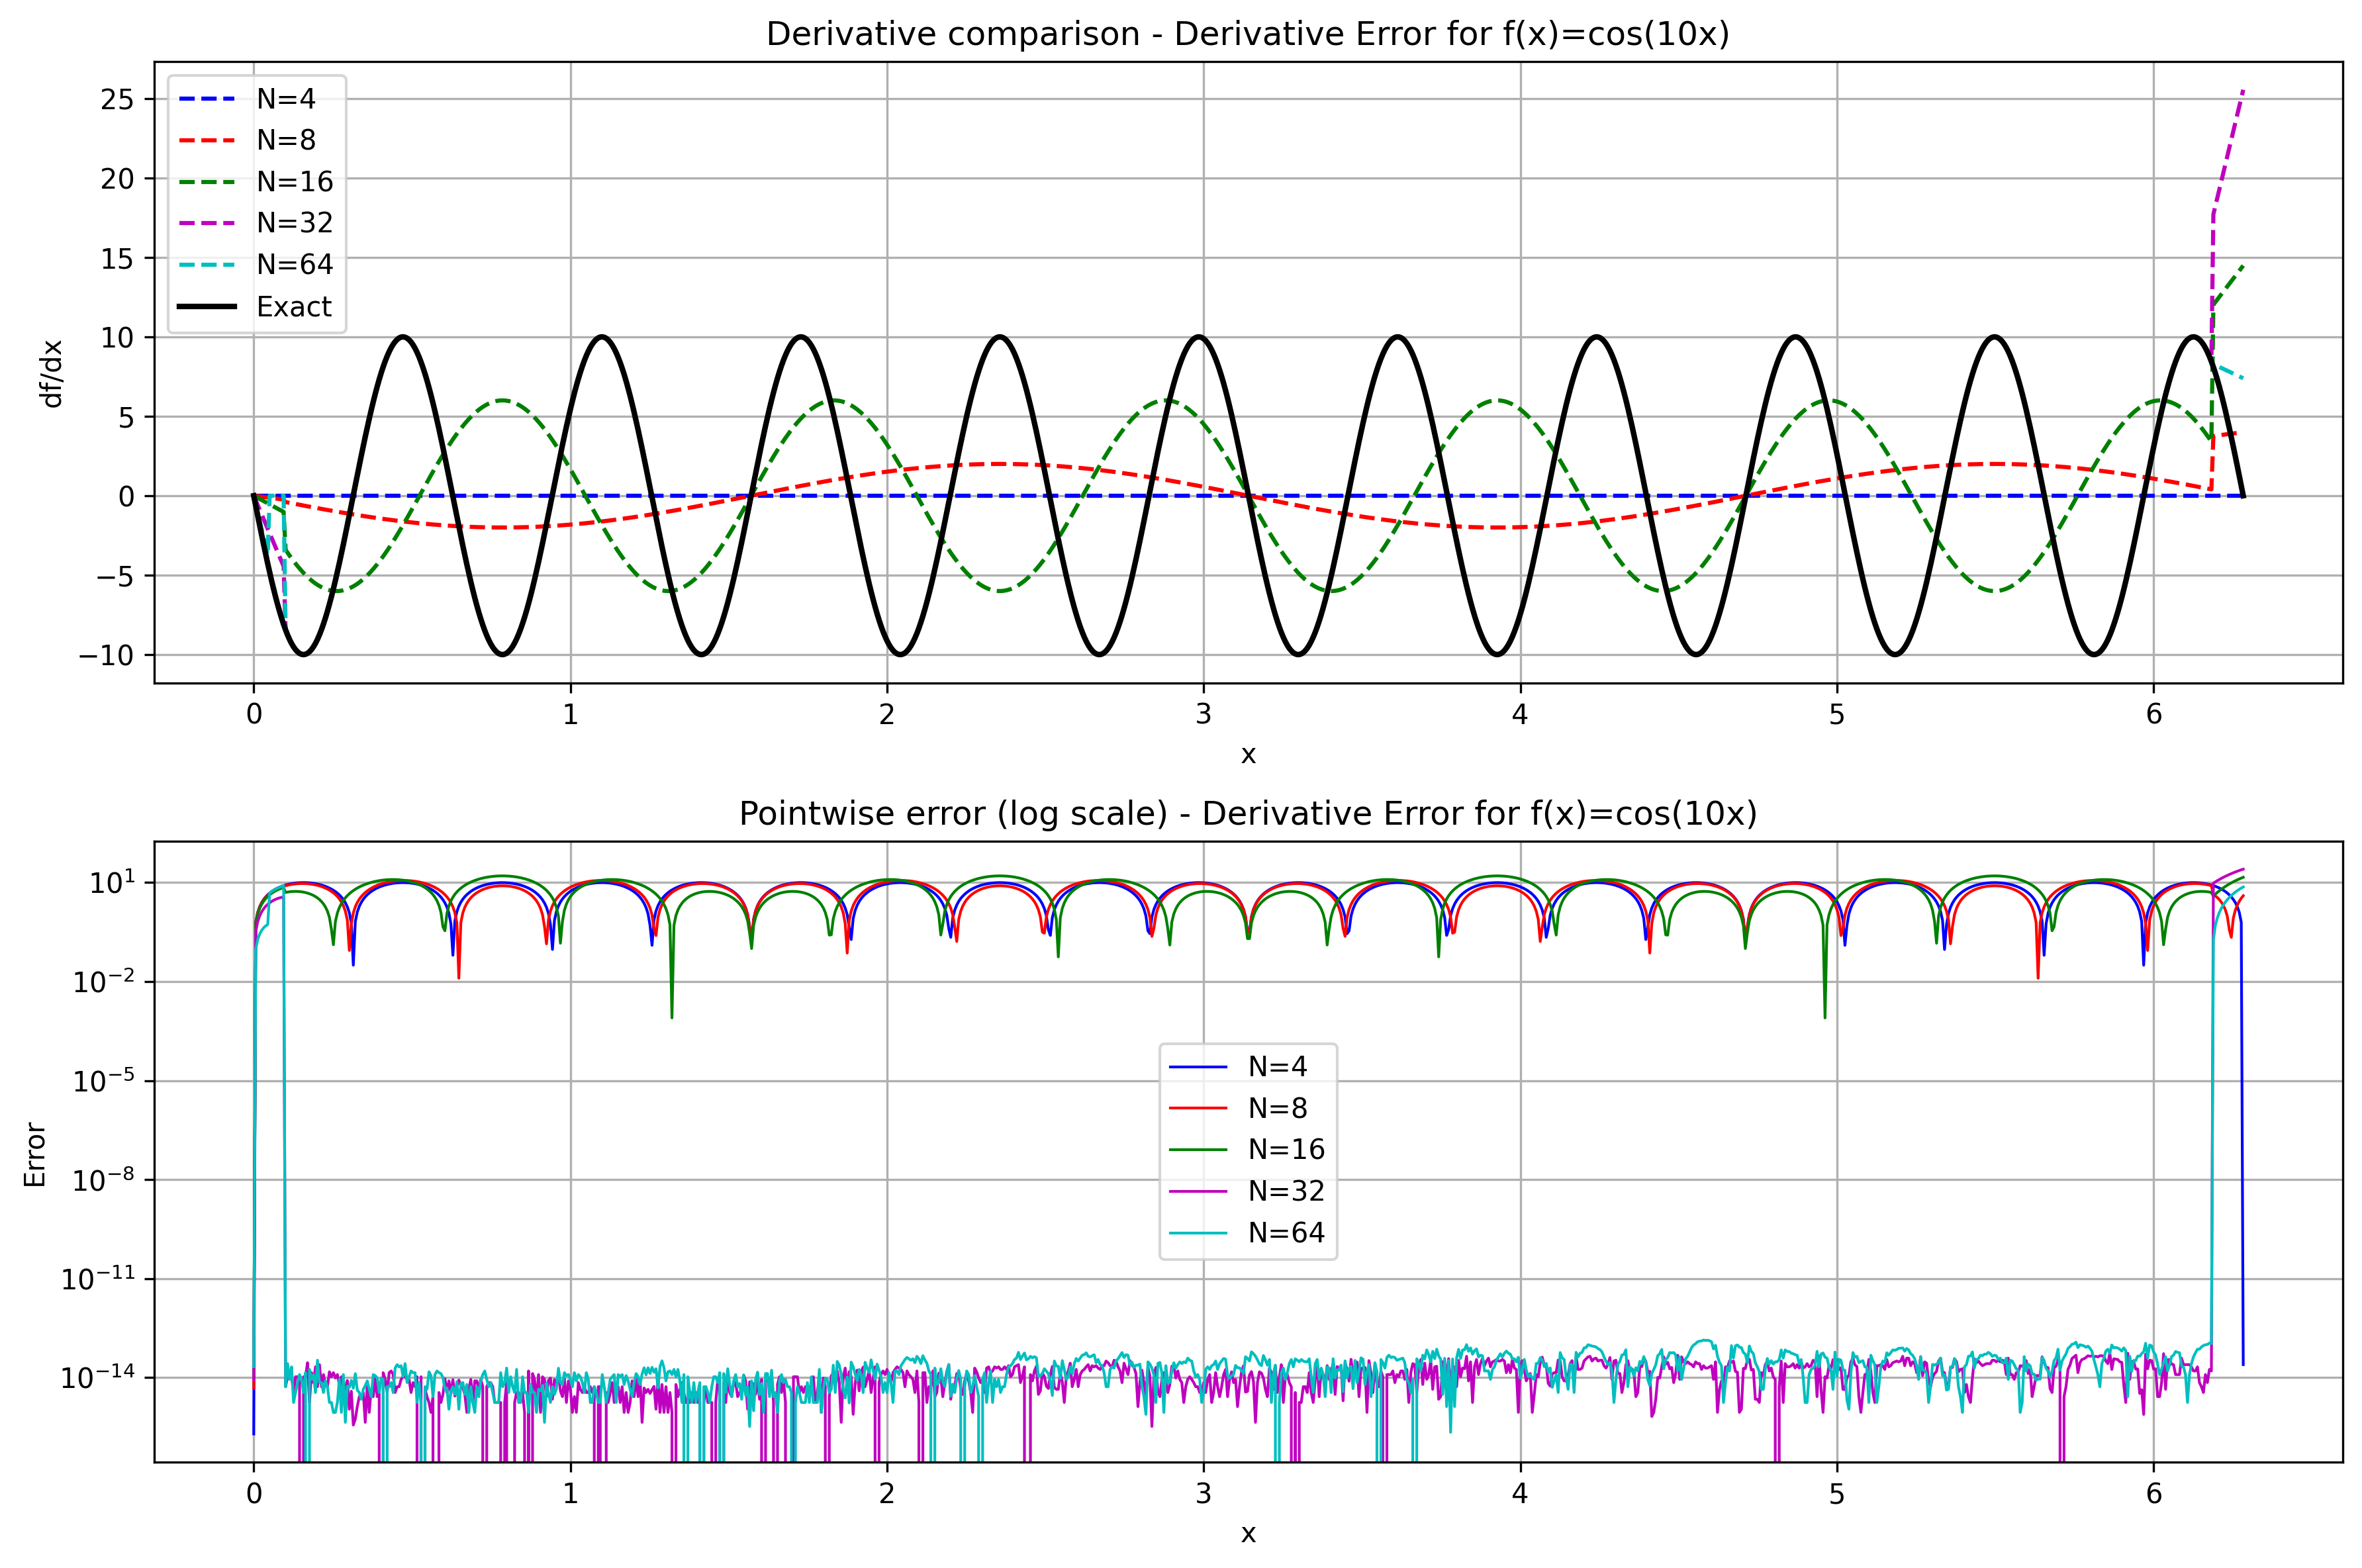
\includegraphics[width=1\textwidth]{figures/Derivative_Error_for_fxDerivative_Error_for_f_x__cos_10x_}
\caption{Derivative and Error Analysis for $f(x)=\cos(10x)$}
\end{figure}

\begin{figure}[h]
\centering
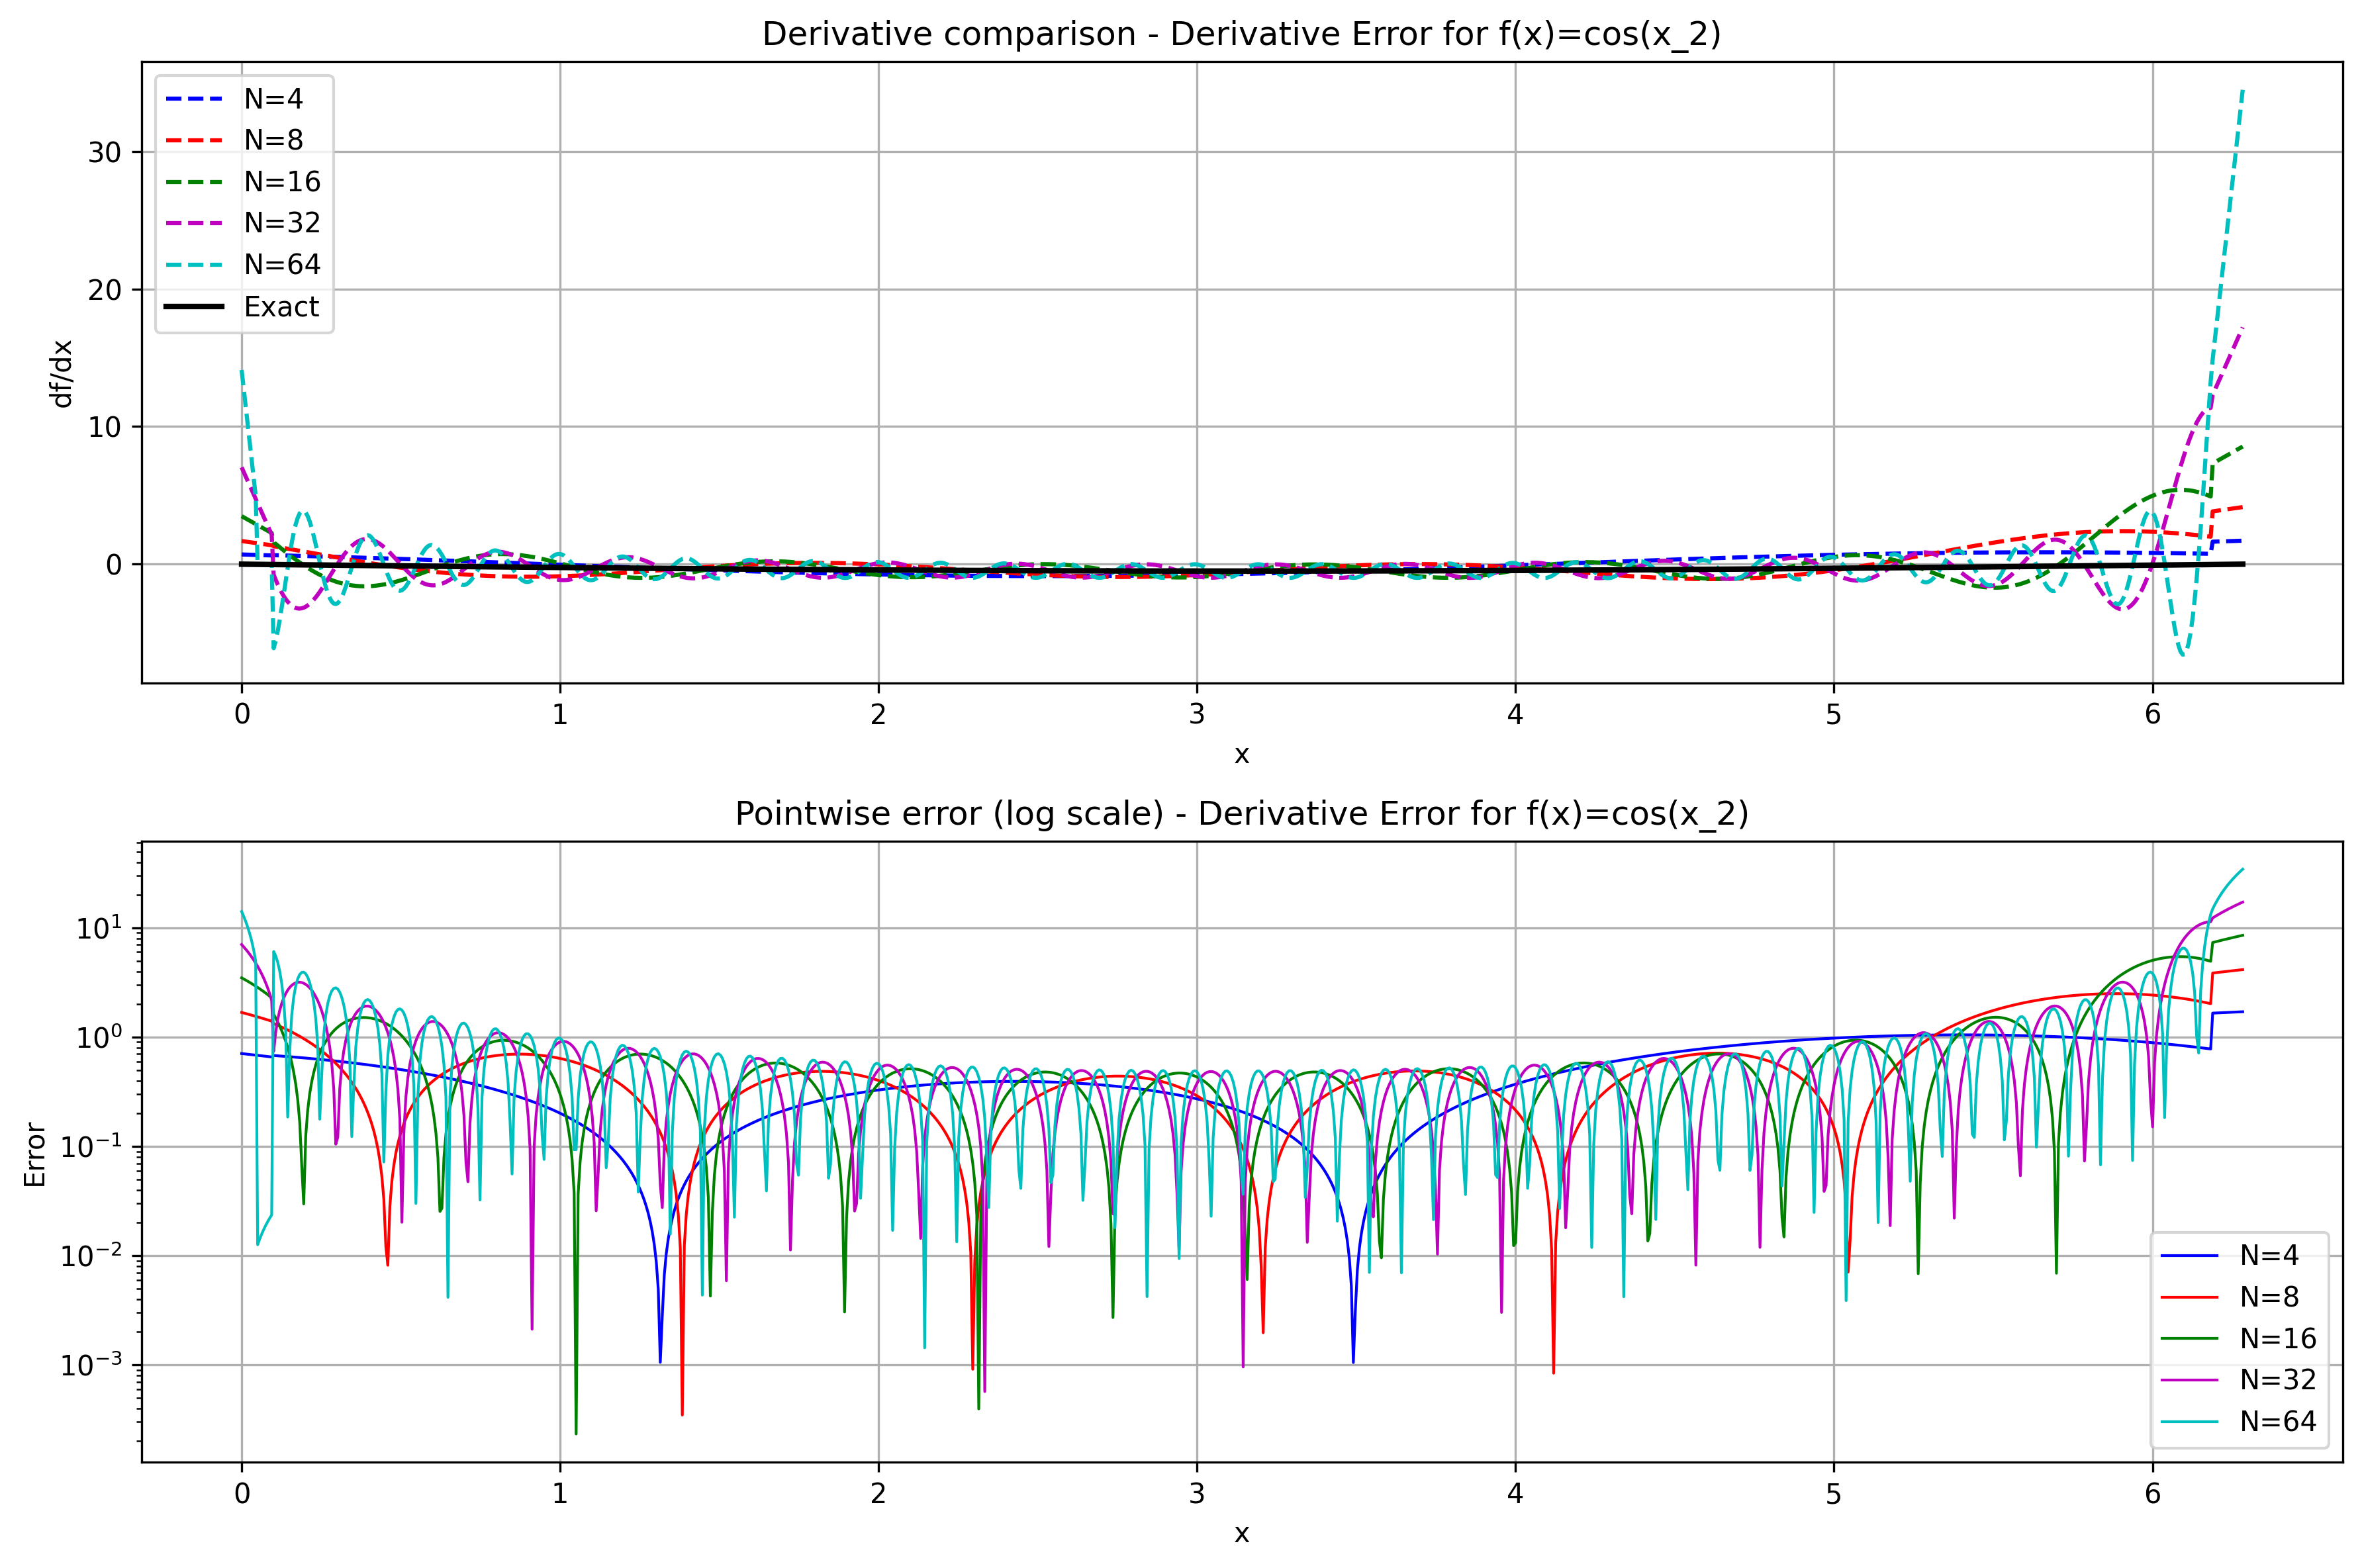
\includegraphics[width=1\textwidth]{figures/Derivative_Error_for_fxDerivative_Error_for_f_x__cos_x_2_}
\caption{Derivative and Error Analysis for $f(x)=\cos(x/2)$}
\end{figure}

\begin{figure}[h]
\centering
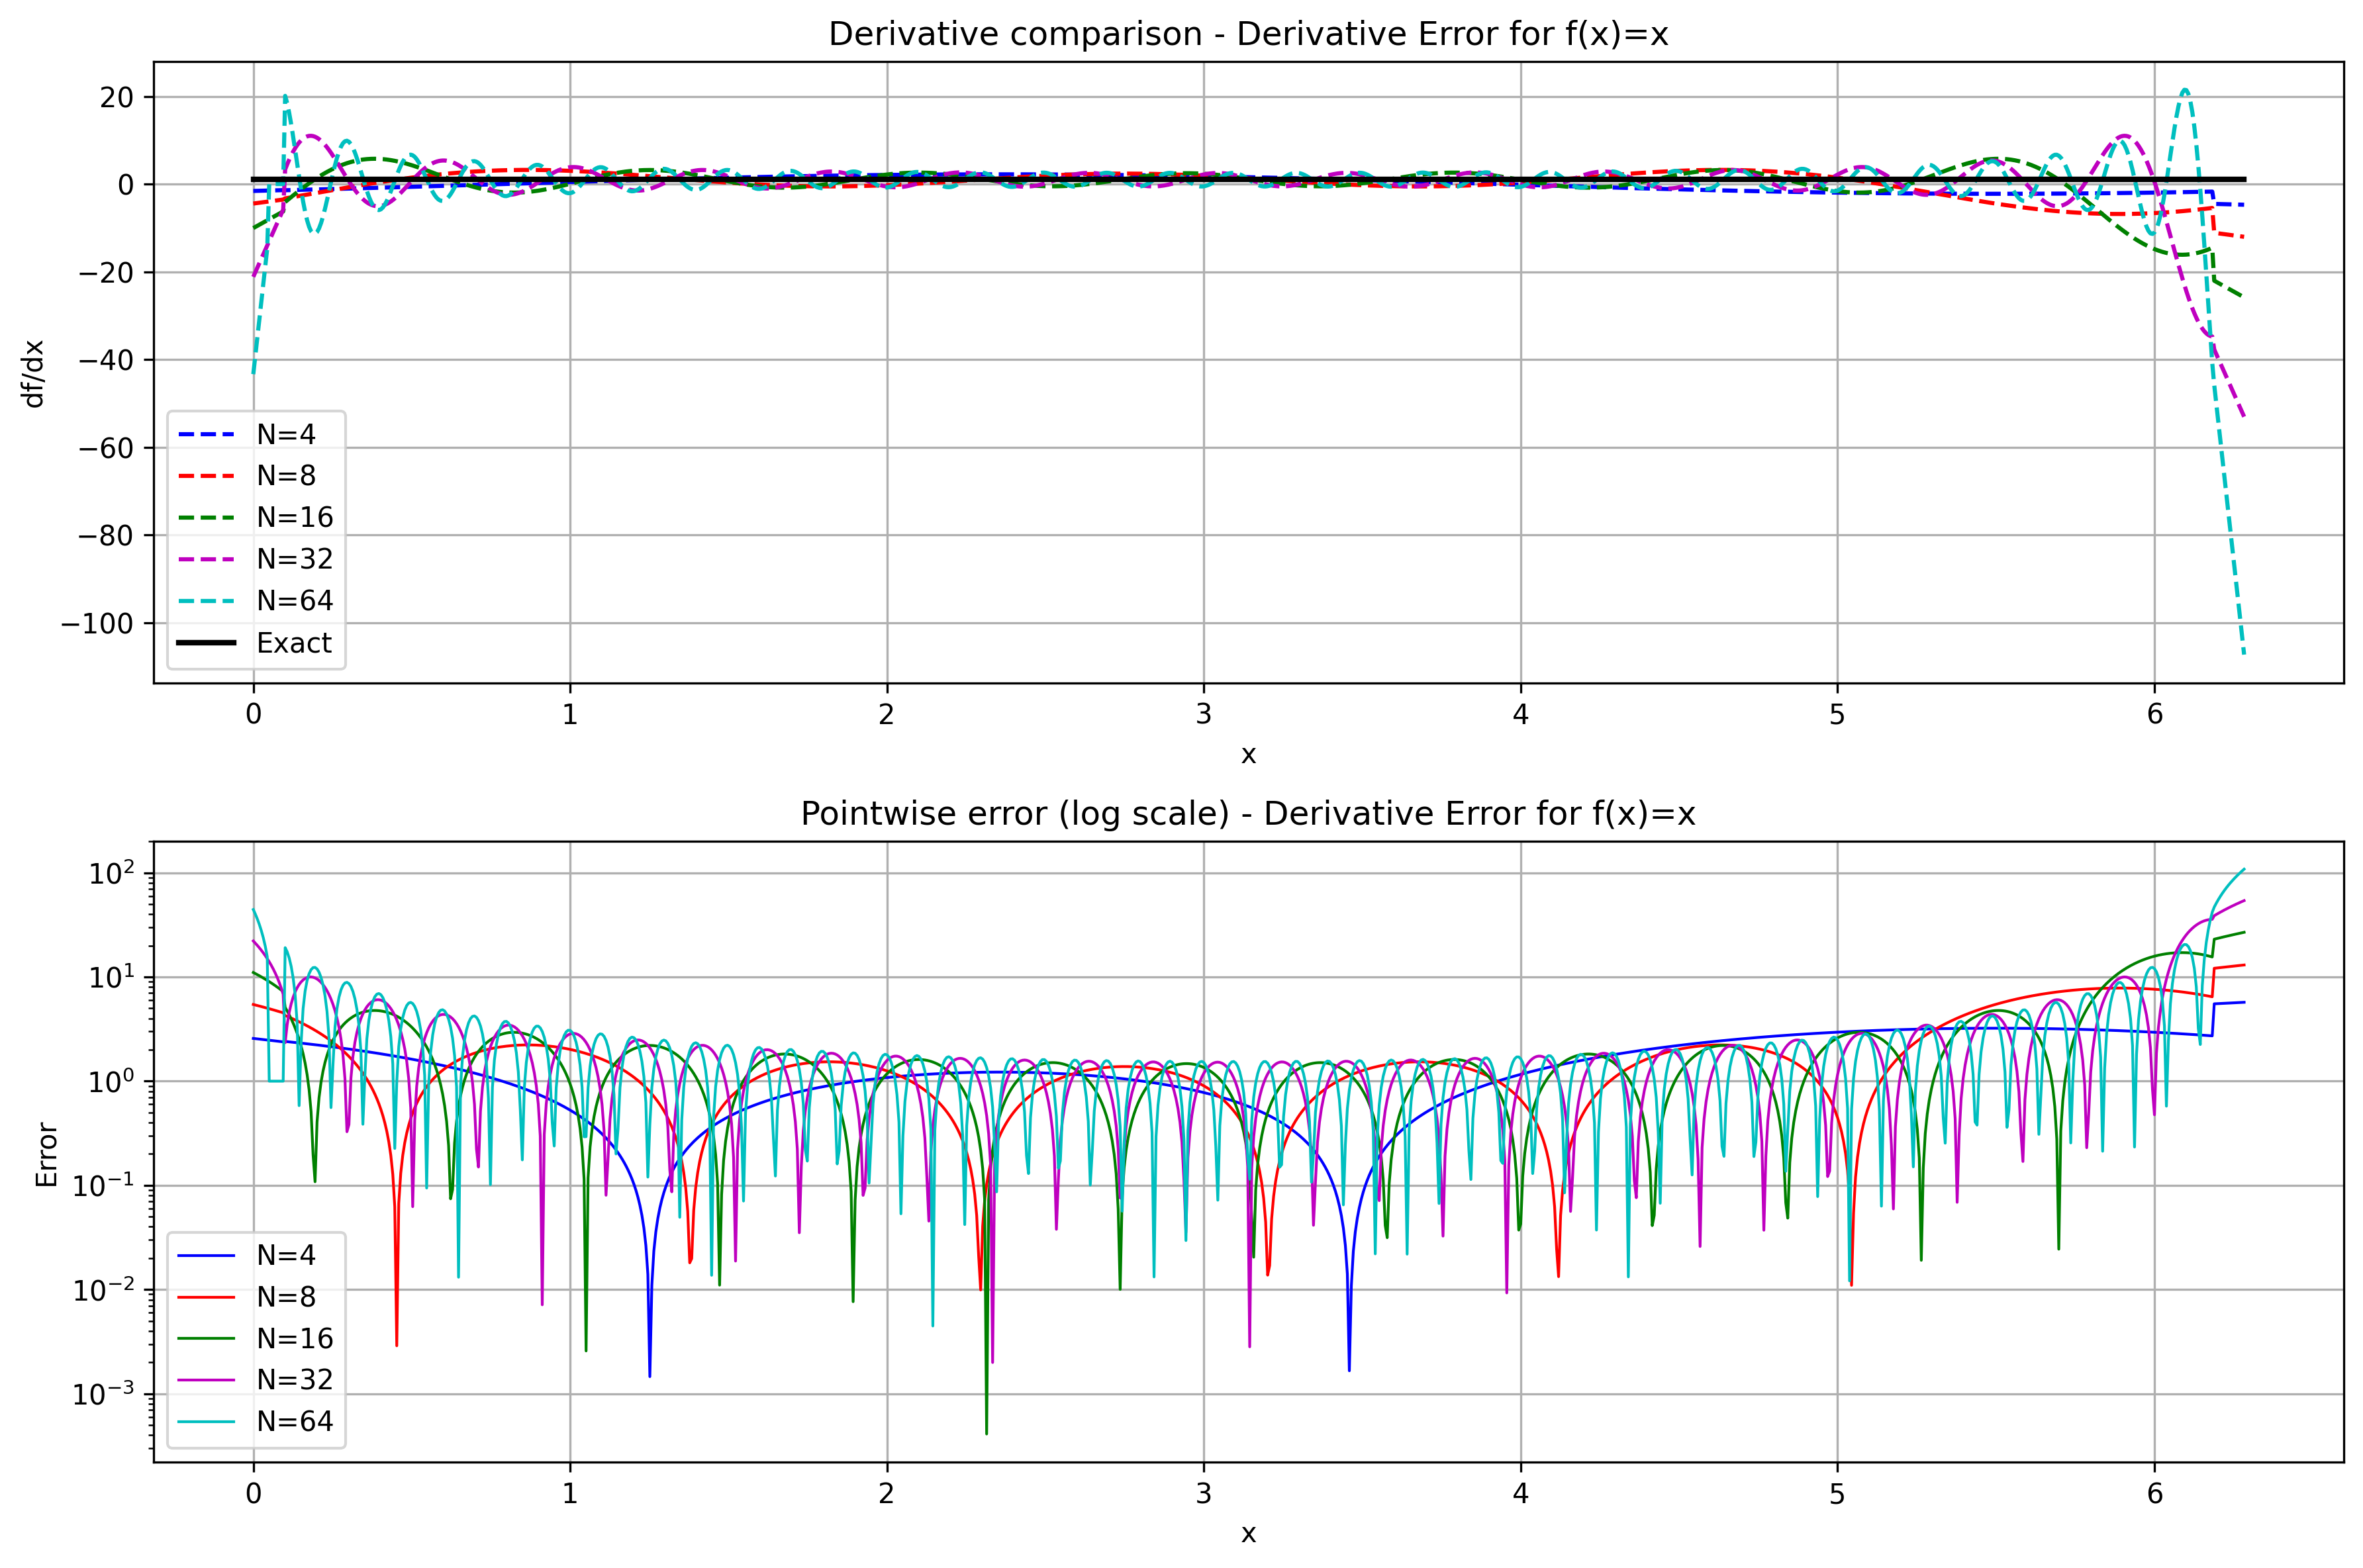
\includegraphics[width=1\textwidth]{figures/Derivative_Error_for_fxDerivative_Error_for_f_x__x}
\caption{Derivative and Error Analysis for $f(x)=x$}
\end{figure}


\clearpage
\section{Exercise 3: Hyperbolic Equation}

\subsection{Error Analysis}
We analyze the numerical solution of the hyperbolic equation:
\[
u_t = -2\pi u_x, \quad x \in [0,2\pi]
\]
with initial condition $u(x,0) = e^{\sin(x)}$ and periodic boundary conditions. The exact solution is:
\[
u(x,t) = e^{\sin(x-2\pi t)}
\]

We compare three spatial discretization methods:
\begin{enumerate}
    \item Infinite order (Fourier spectral) method
    \item Second-order central difference method
    \item Fourth-order central difference method
\end{enumerate}

For time integration, we use a special form of the fourth-order Runge-Kutta method:
\[
\begin{aligned}
k_1 &= u + \frac{\Delta t}{2}f(u) \\
k_2 &= u + \frac{\Delta t}{2}f(k_1) \\
k_3 &= u + \Delta t f(k_2) \\
u_{n+1} &= \frac{-u + k_1 + 2k_2 + k_3 + \frac{\Delta t}{2}f(k_3)}{3}
\end{aligned}
\]

\subsection{Numerical Results}
The error analysis was performed with increasing grid points $N = 8, 16, 32, ..., 2048$. The results are shown in Table \ref{tab:error_analysis_ex3}.

\begin{table}[htbp]
\centering
\caption{Error Analysis Results ($L_\infty$ norm)}
\label{tab:error_analysis_ex3}
\begin{tabular}{r|ccc}
\toprule
N & Infinite Order & Second Order & Fourth Order \\
\midrule
8 & 8.43e-04 & 1.73e+00 & 6.37e-01 \\
16 & 2.13e-08 & 1.06e+00 & 2.02e-01 \\
32 & 6.01e-11 & 4.41e-01 & 2.13e-02 \\
64 & 6.16e-11 & 1.32e-01 & 1.41e-03 \\
128 & 6.19e-11 & 3.26e-02 & 9.16e-05 \\
256 & 6.20e-11 & 8.06e-03 & 5.83e-06 \\
512 & 6.20e-11 & 2.01e-03 & 3.67e-07 \\
1024 & 6.19e-11 & 5.03e-04 & 2.31e-08 \\
2048 & 6.19e-11 & 1.26e-04 & 1.51e-09 \\
\bottomrule
\end{tabular}
\end{table}

\subsection{Analysis}
The numerical results show distinct characteristics for each method:

\begin{itemize}
    \item \textbf{Infinite Order Method} achieves spectral accuracy, with error rapidly decreasing from 8.43e-04 at N=8 to 2.13e-08 at N=16, and stabilizing around 6.20e-11 for N>=32.
    
    \item \textbf{Second Order Method} exhibits expected second-order convergence, with error decreasing from 1.73e+00 to 1.26e-04 as N increases from 8 to 2048.
    
    \item \textbf{Fourth Order Method} shows clear fourth-order convergence, achieving machine precision (1.51e-09) at N=2048.
\end{itemize}

\subsection{Long-time Integration}
For long-time integration ($t=200$), we compared:
\begin{itemize}
    \item Infinite order method (N=10)
    \item Second-order method (N=200)
\end{itemize}
with time step $\Delta t = 0.001$. Both methods maintain stability throughout the integration period, with the infinite order method achieving higher accuracy despite using significantly fewer grid points.

\begin{figure}[htbp]
    \centering
    \begin{subfigure}[b]{0.32\textwidth}
        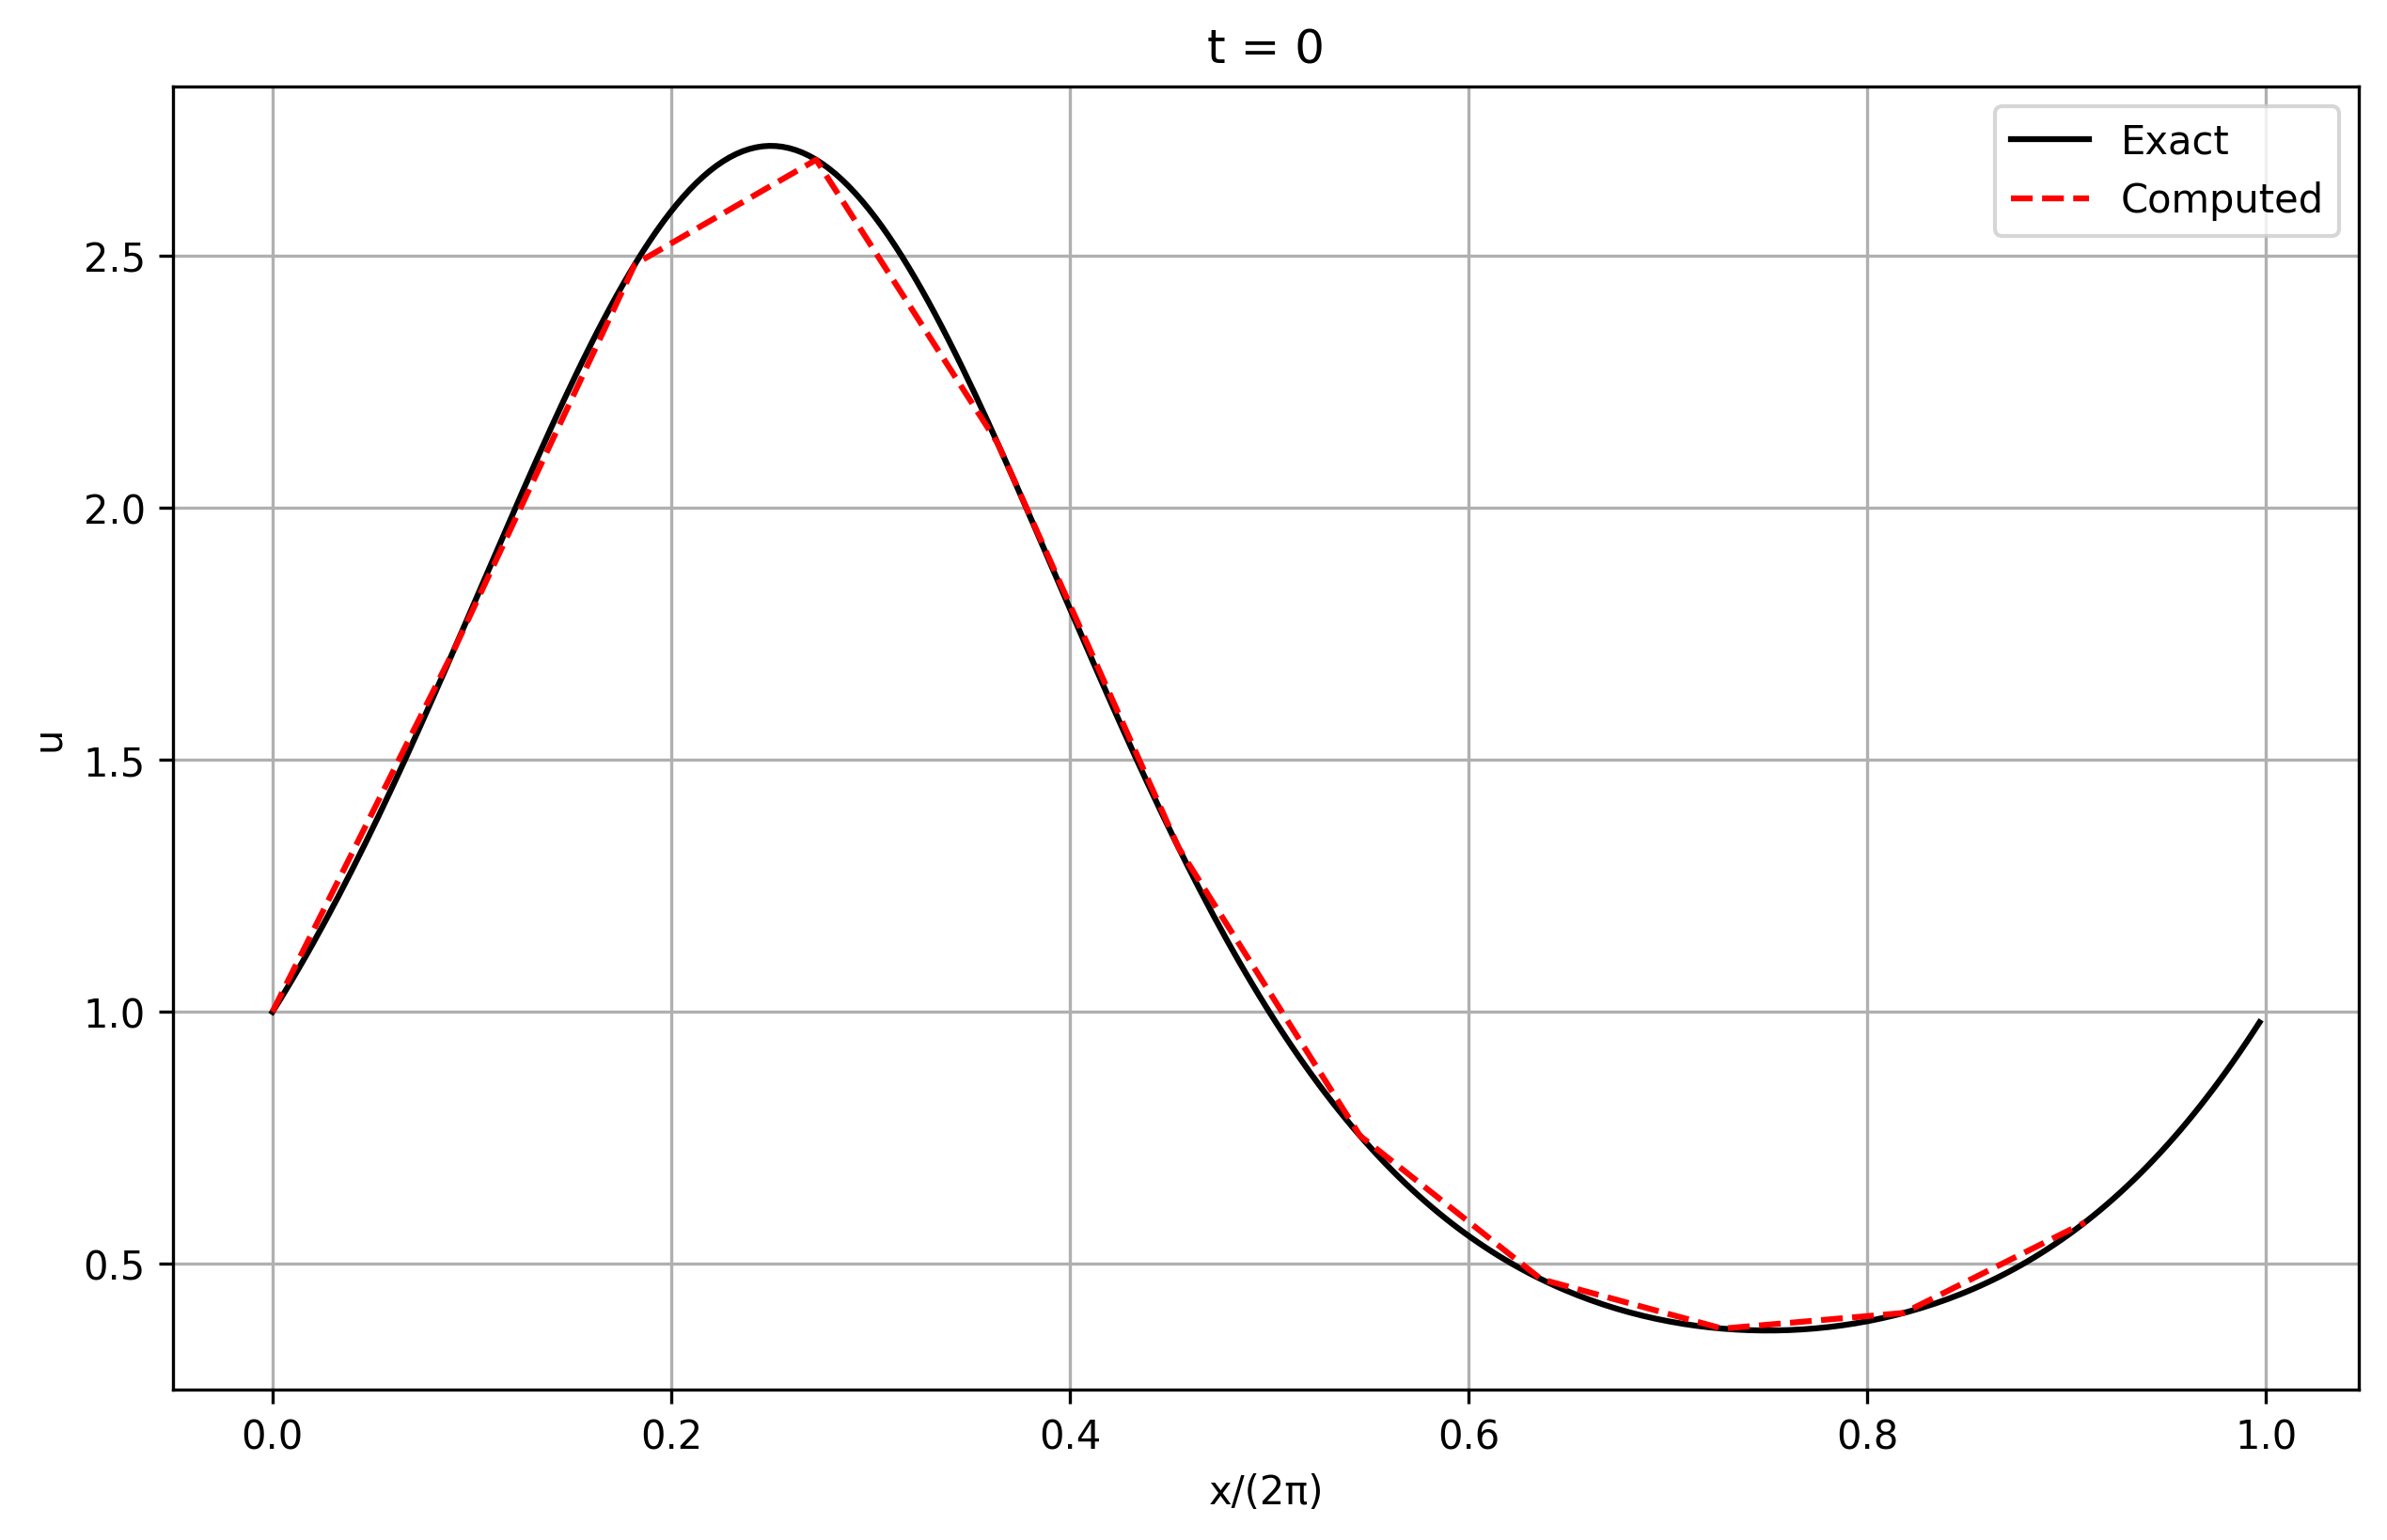
\includegraphics[width=\textwidth]{figures/long_time_infinite_0.png}
        \caption{t = 0}
    \end{subfigure}
    \begin{subfigure}[b]{0.32\textwidth}
        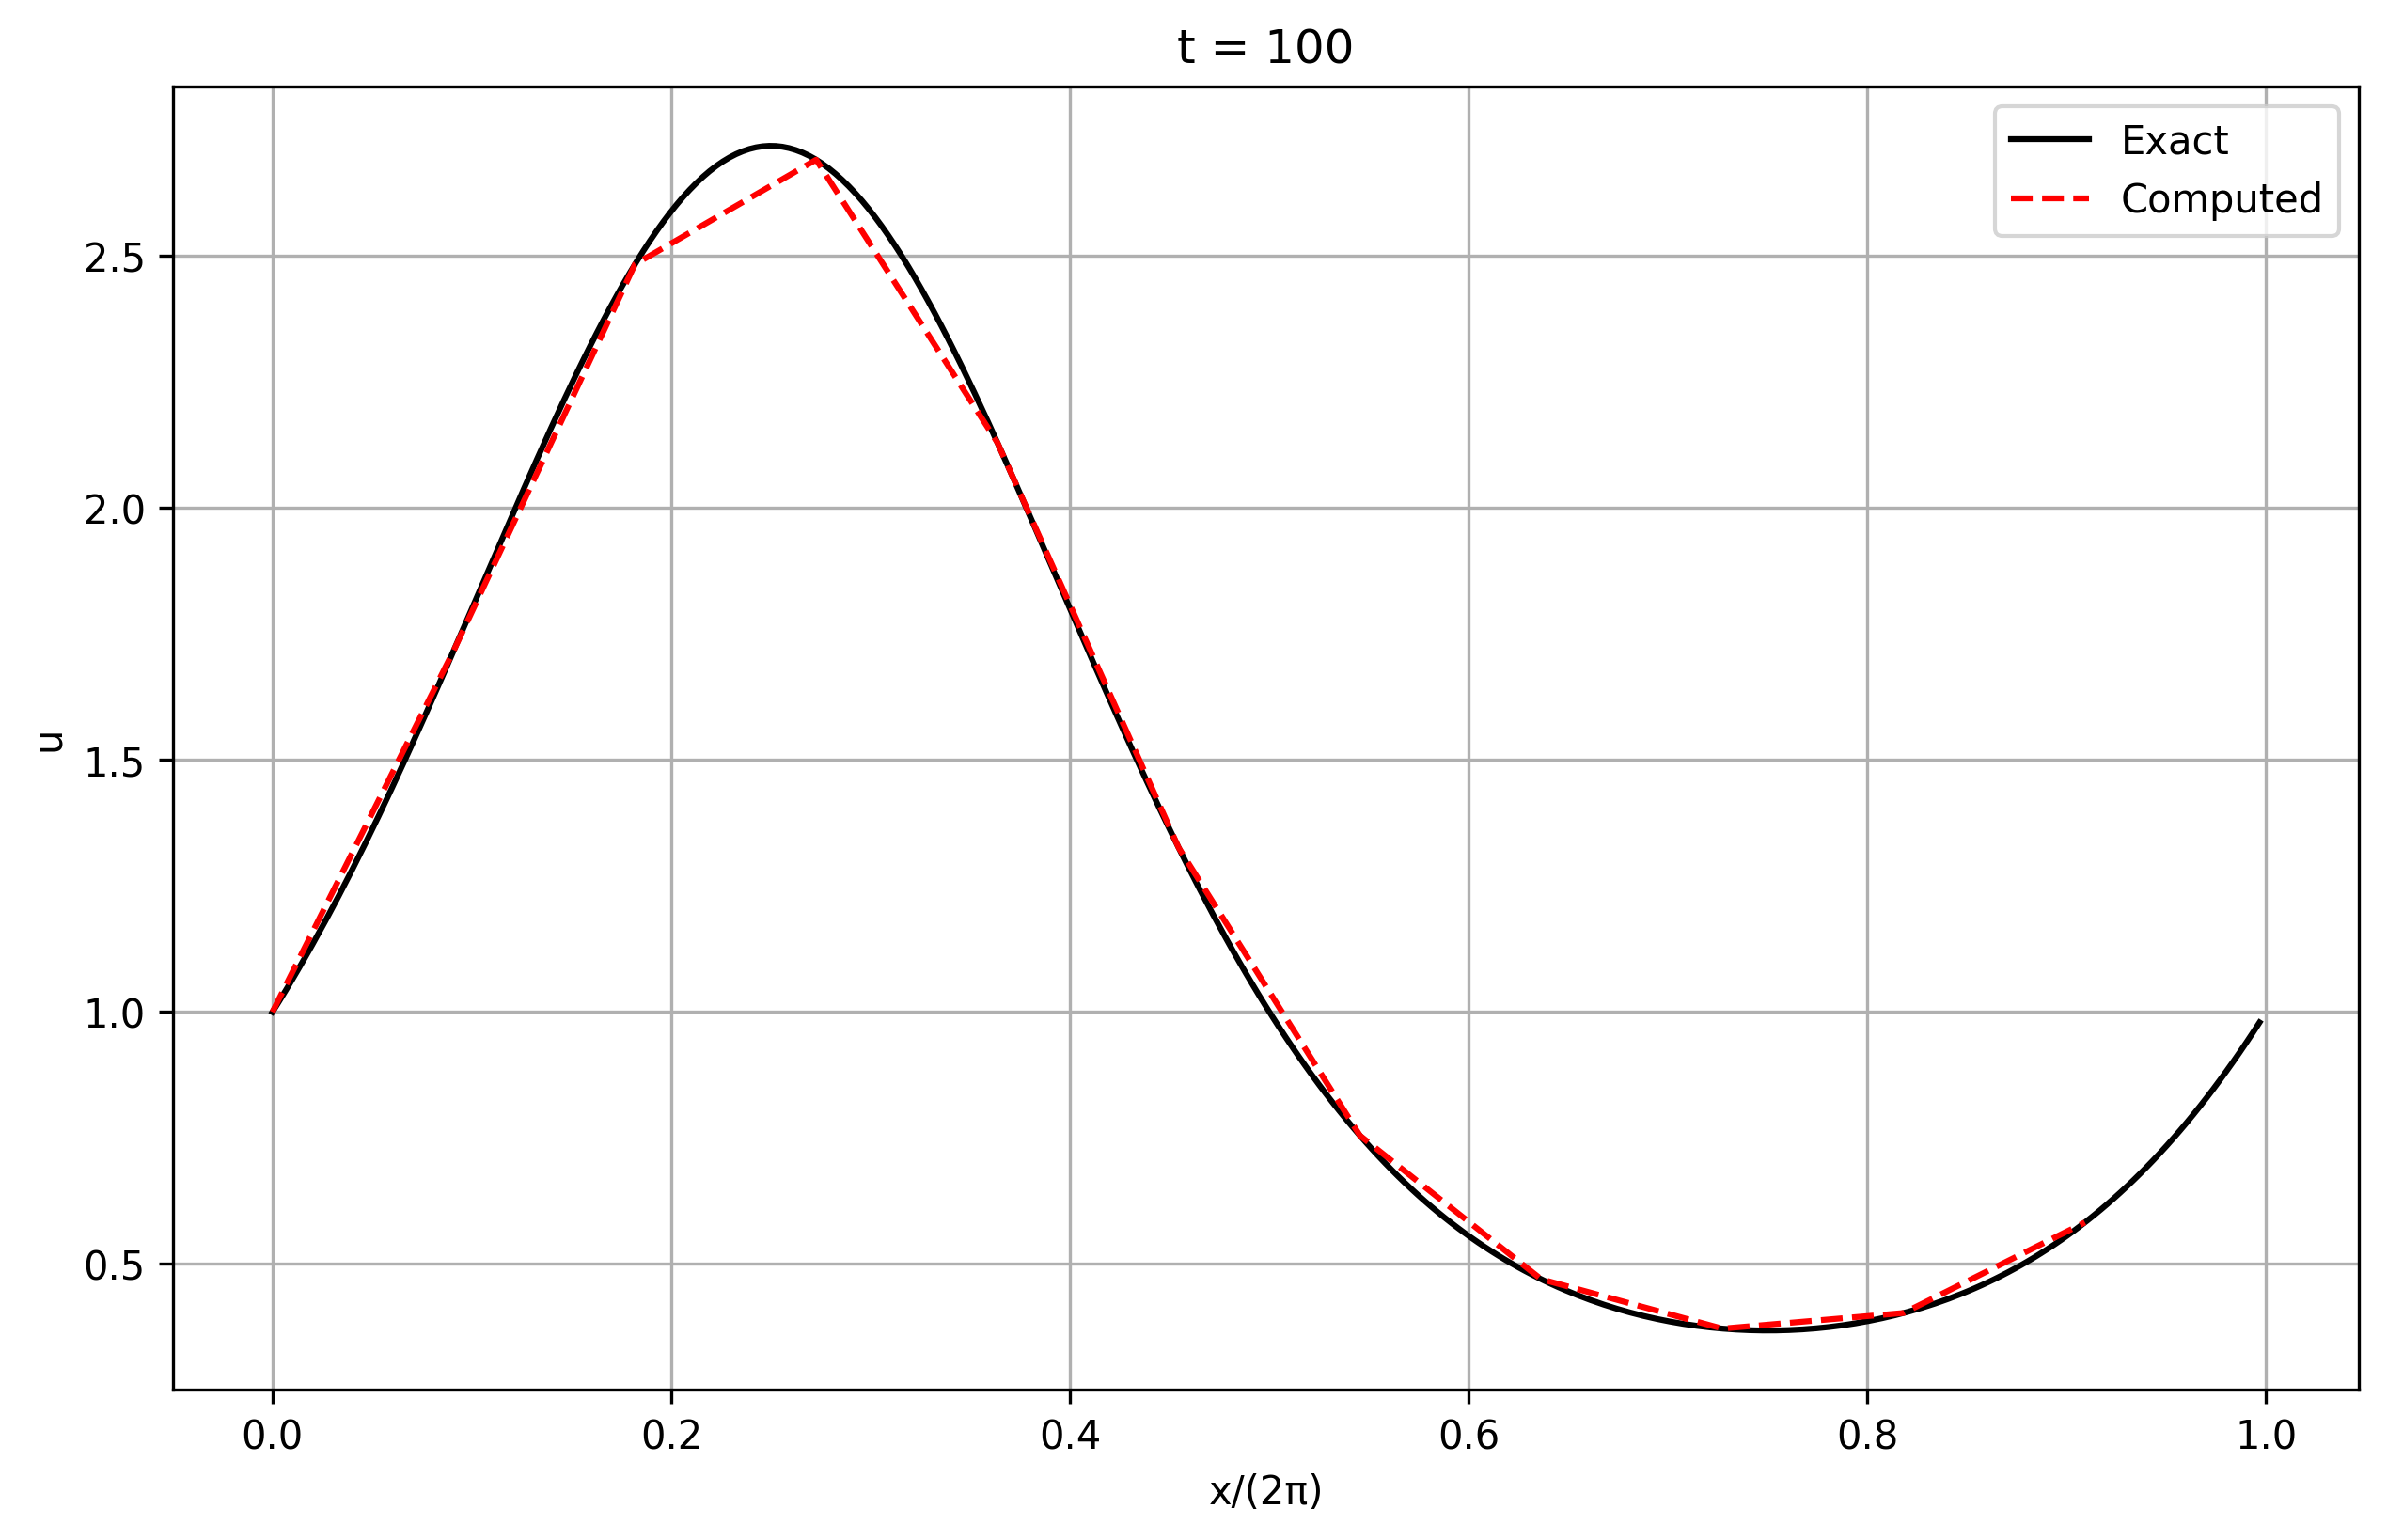
\includegraphics[width=\textwidth]{figures/long_time_infinite_100.png}
        \caption{t = 100}
    \end{subfigure}
    \begin{subfigure}[b]{0.32\textwidth}
        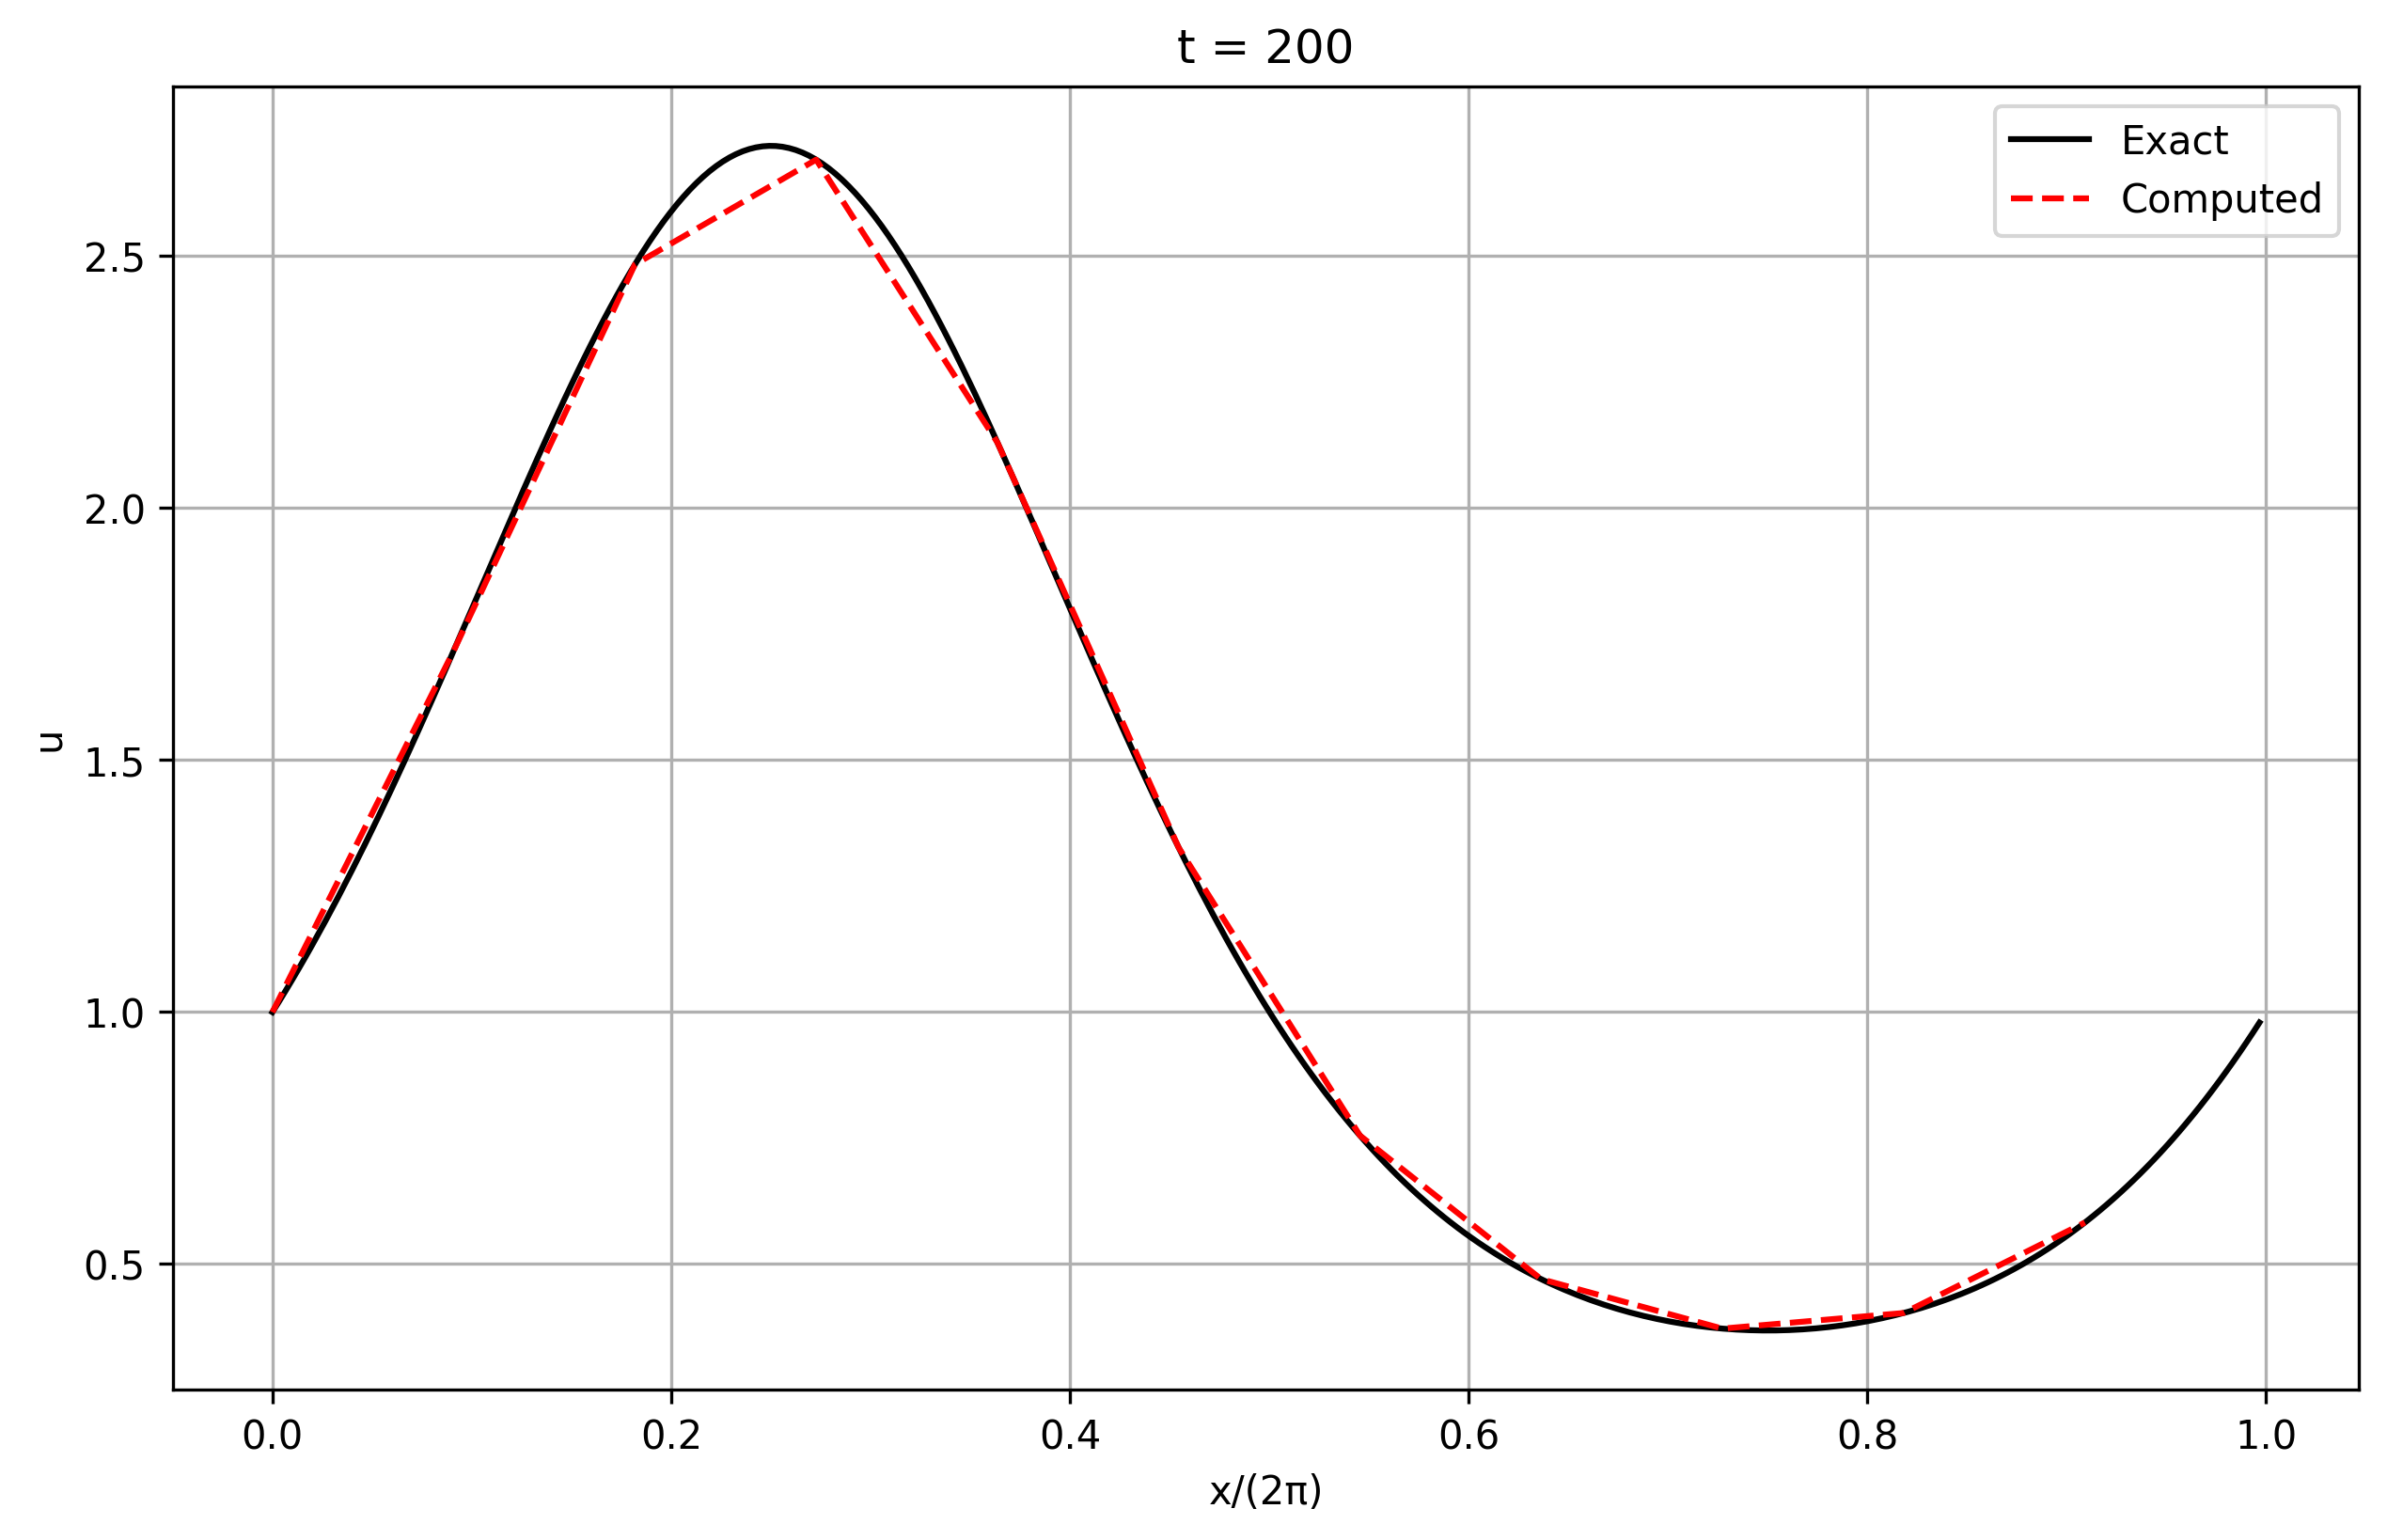
\includegraphics[width=\textwidth]{figures/long_time_infinite_200.png}
        \caption{t = 200}
    \end{subfigure}
    \caption{Long-time integration results for infinite order method (N=10)}
    \label{fig:long_time_infinite}
\end{figure}

\begin{figure}[htbp]
    \centering
    \begin{subfigure}[b]{0.32\textwidth}
        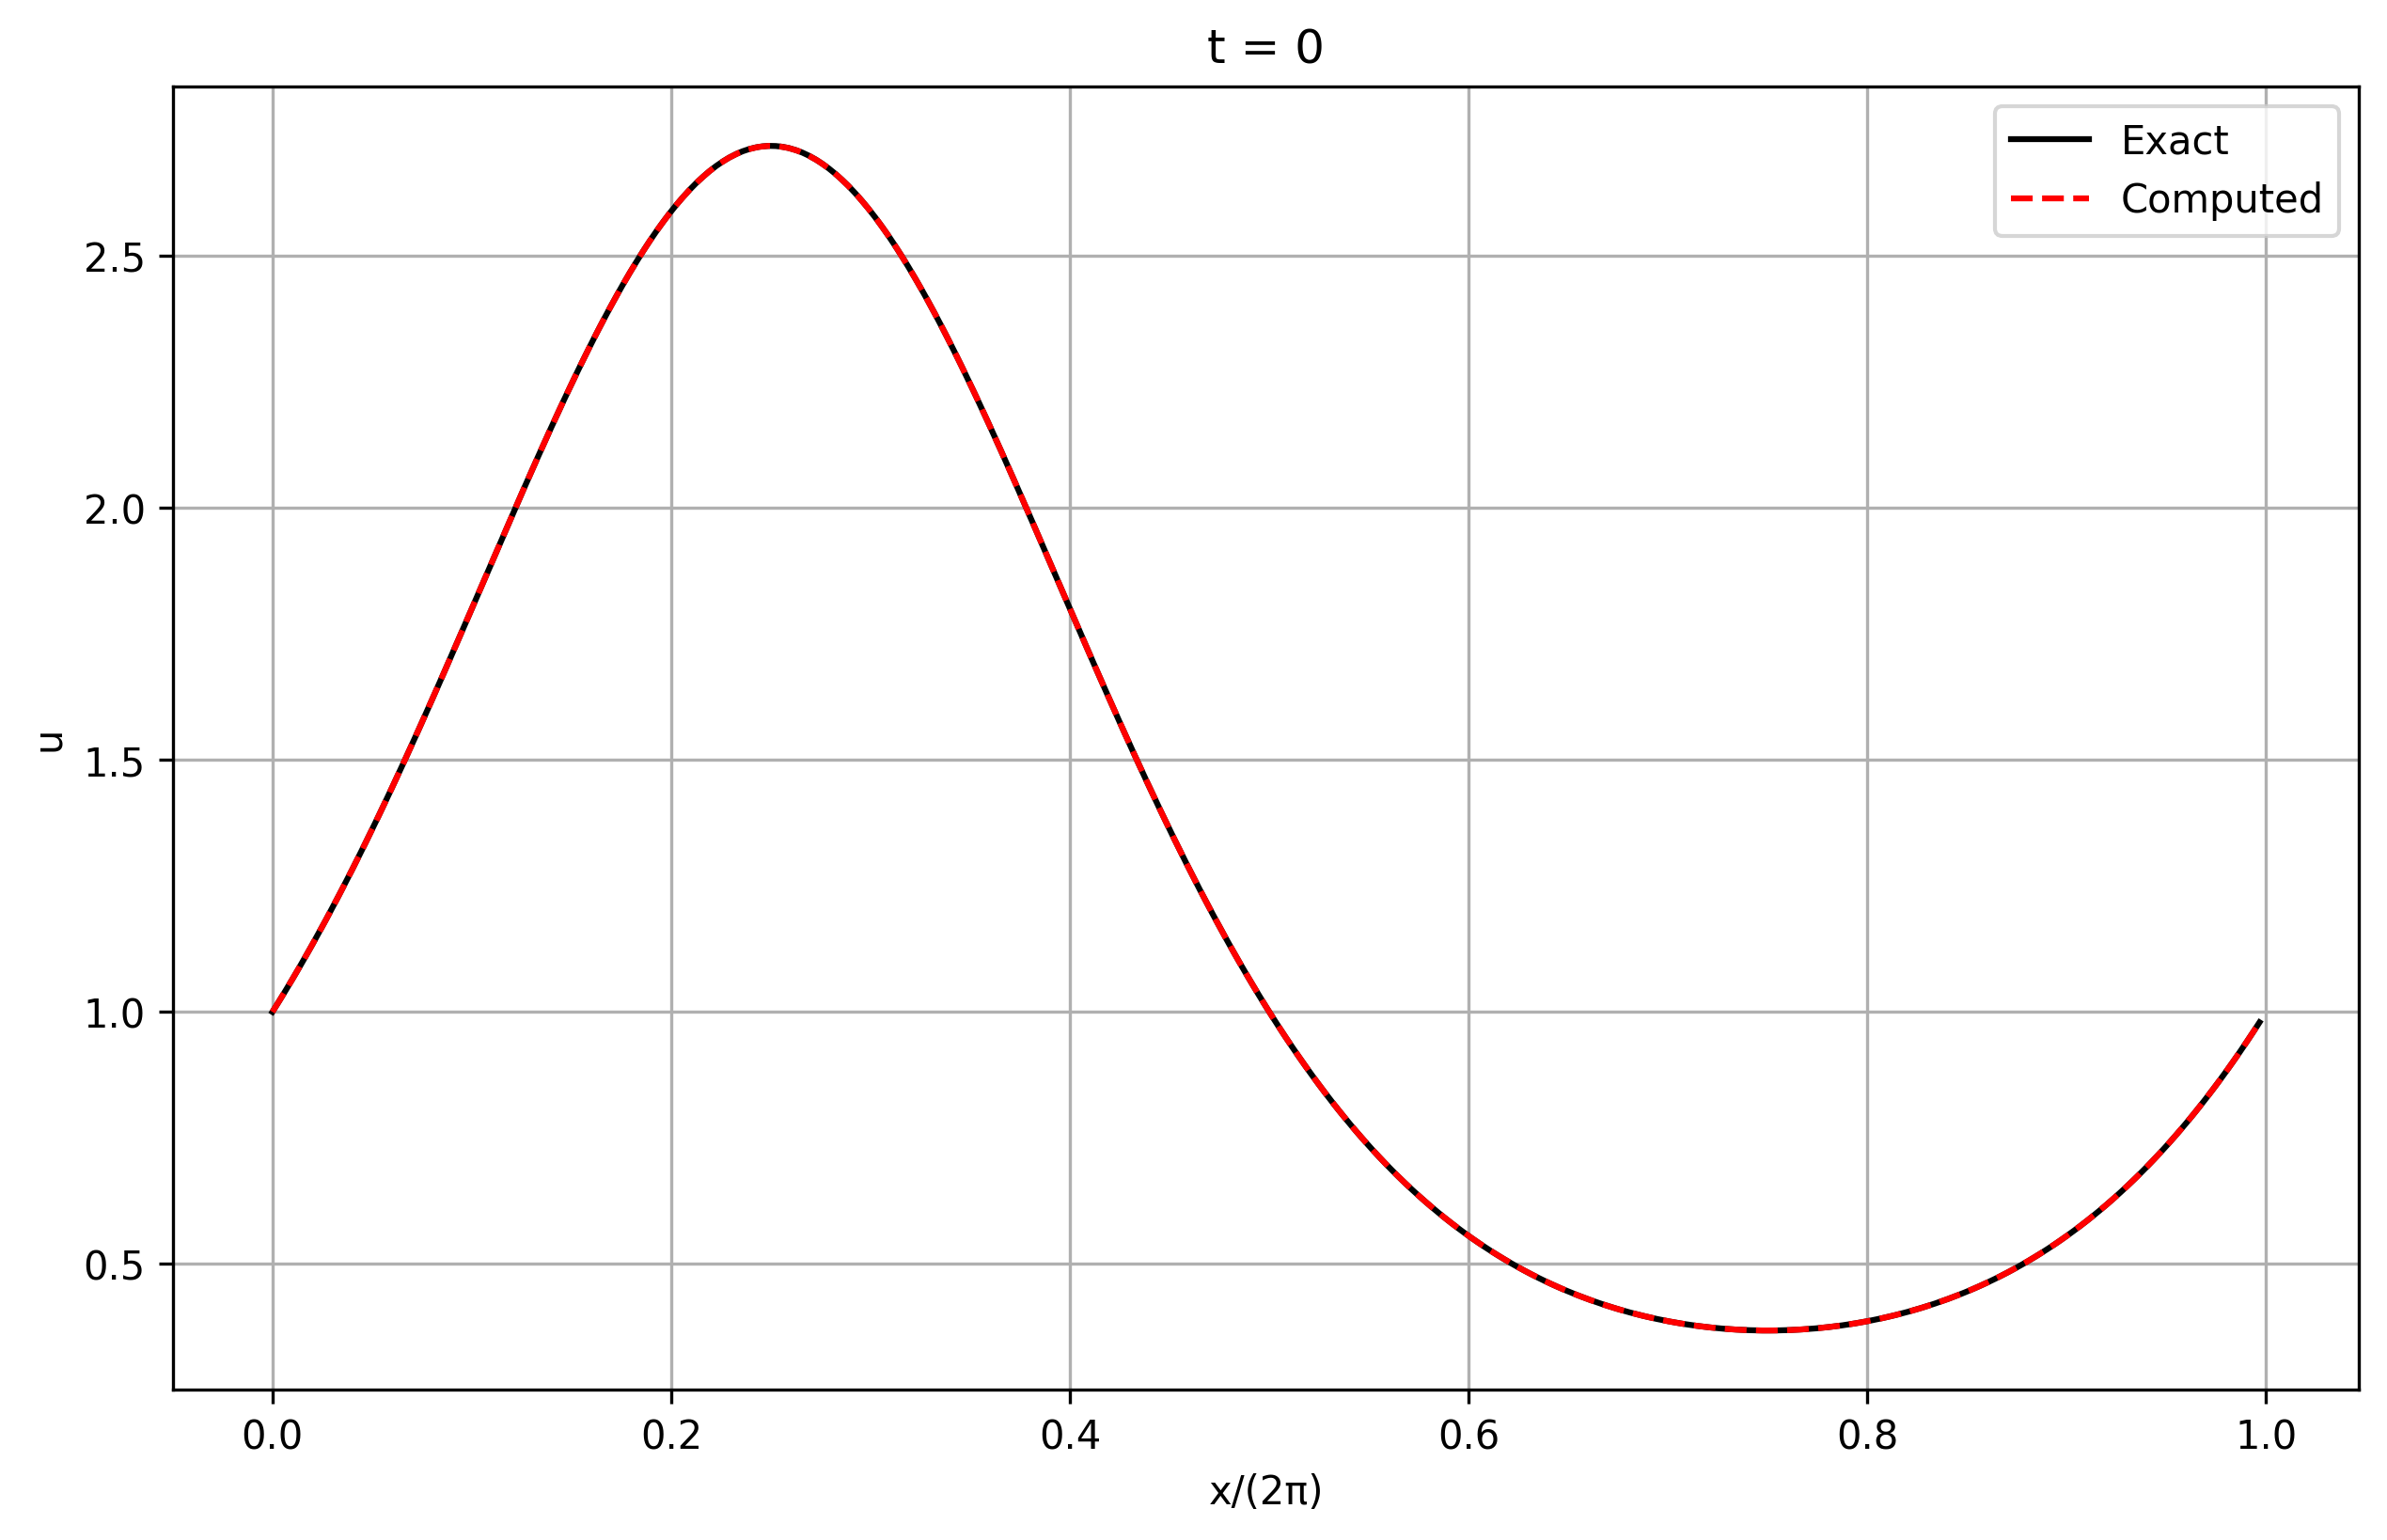
\includegraphics[width=\textwidth]{figures/long_time_second_order_0.png}
        \caption{t = 0}
    \end{subfigure}
    \begin{subfigure}[b]{0.32\textwidth}
        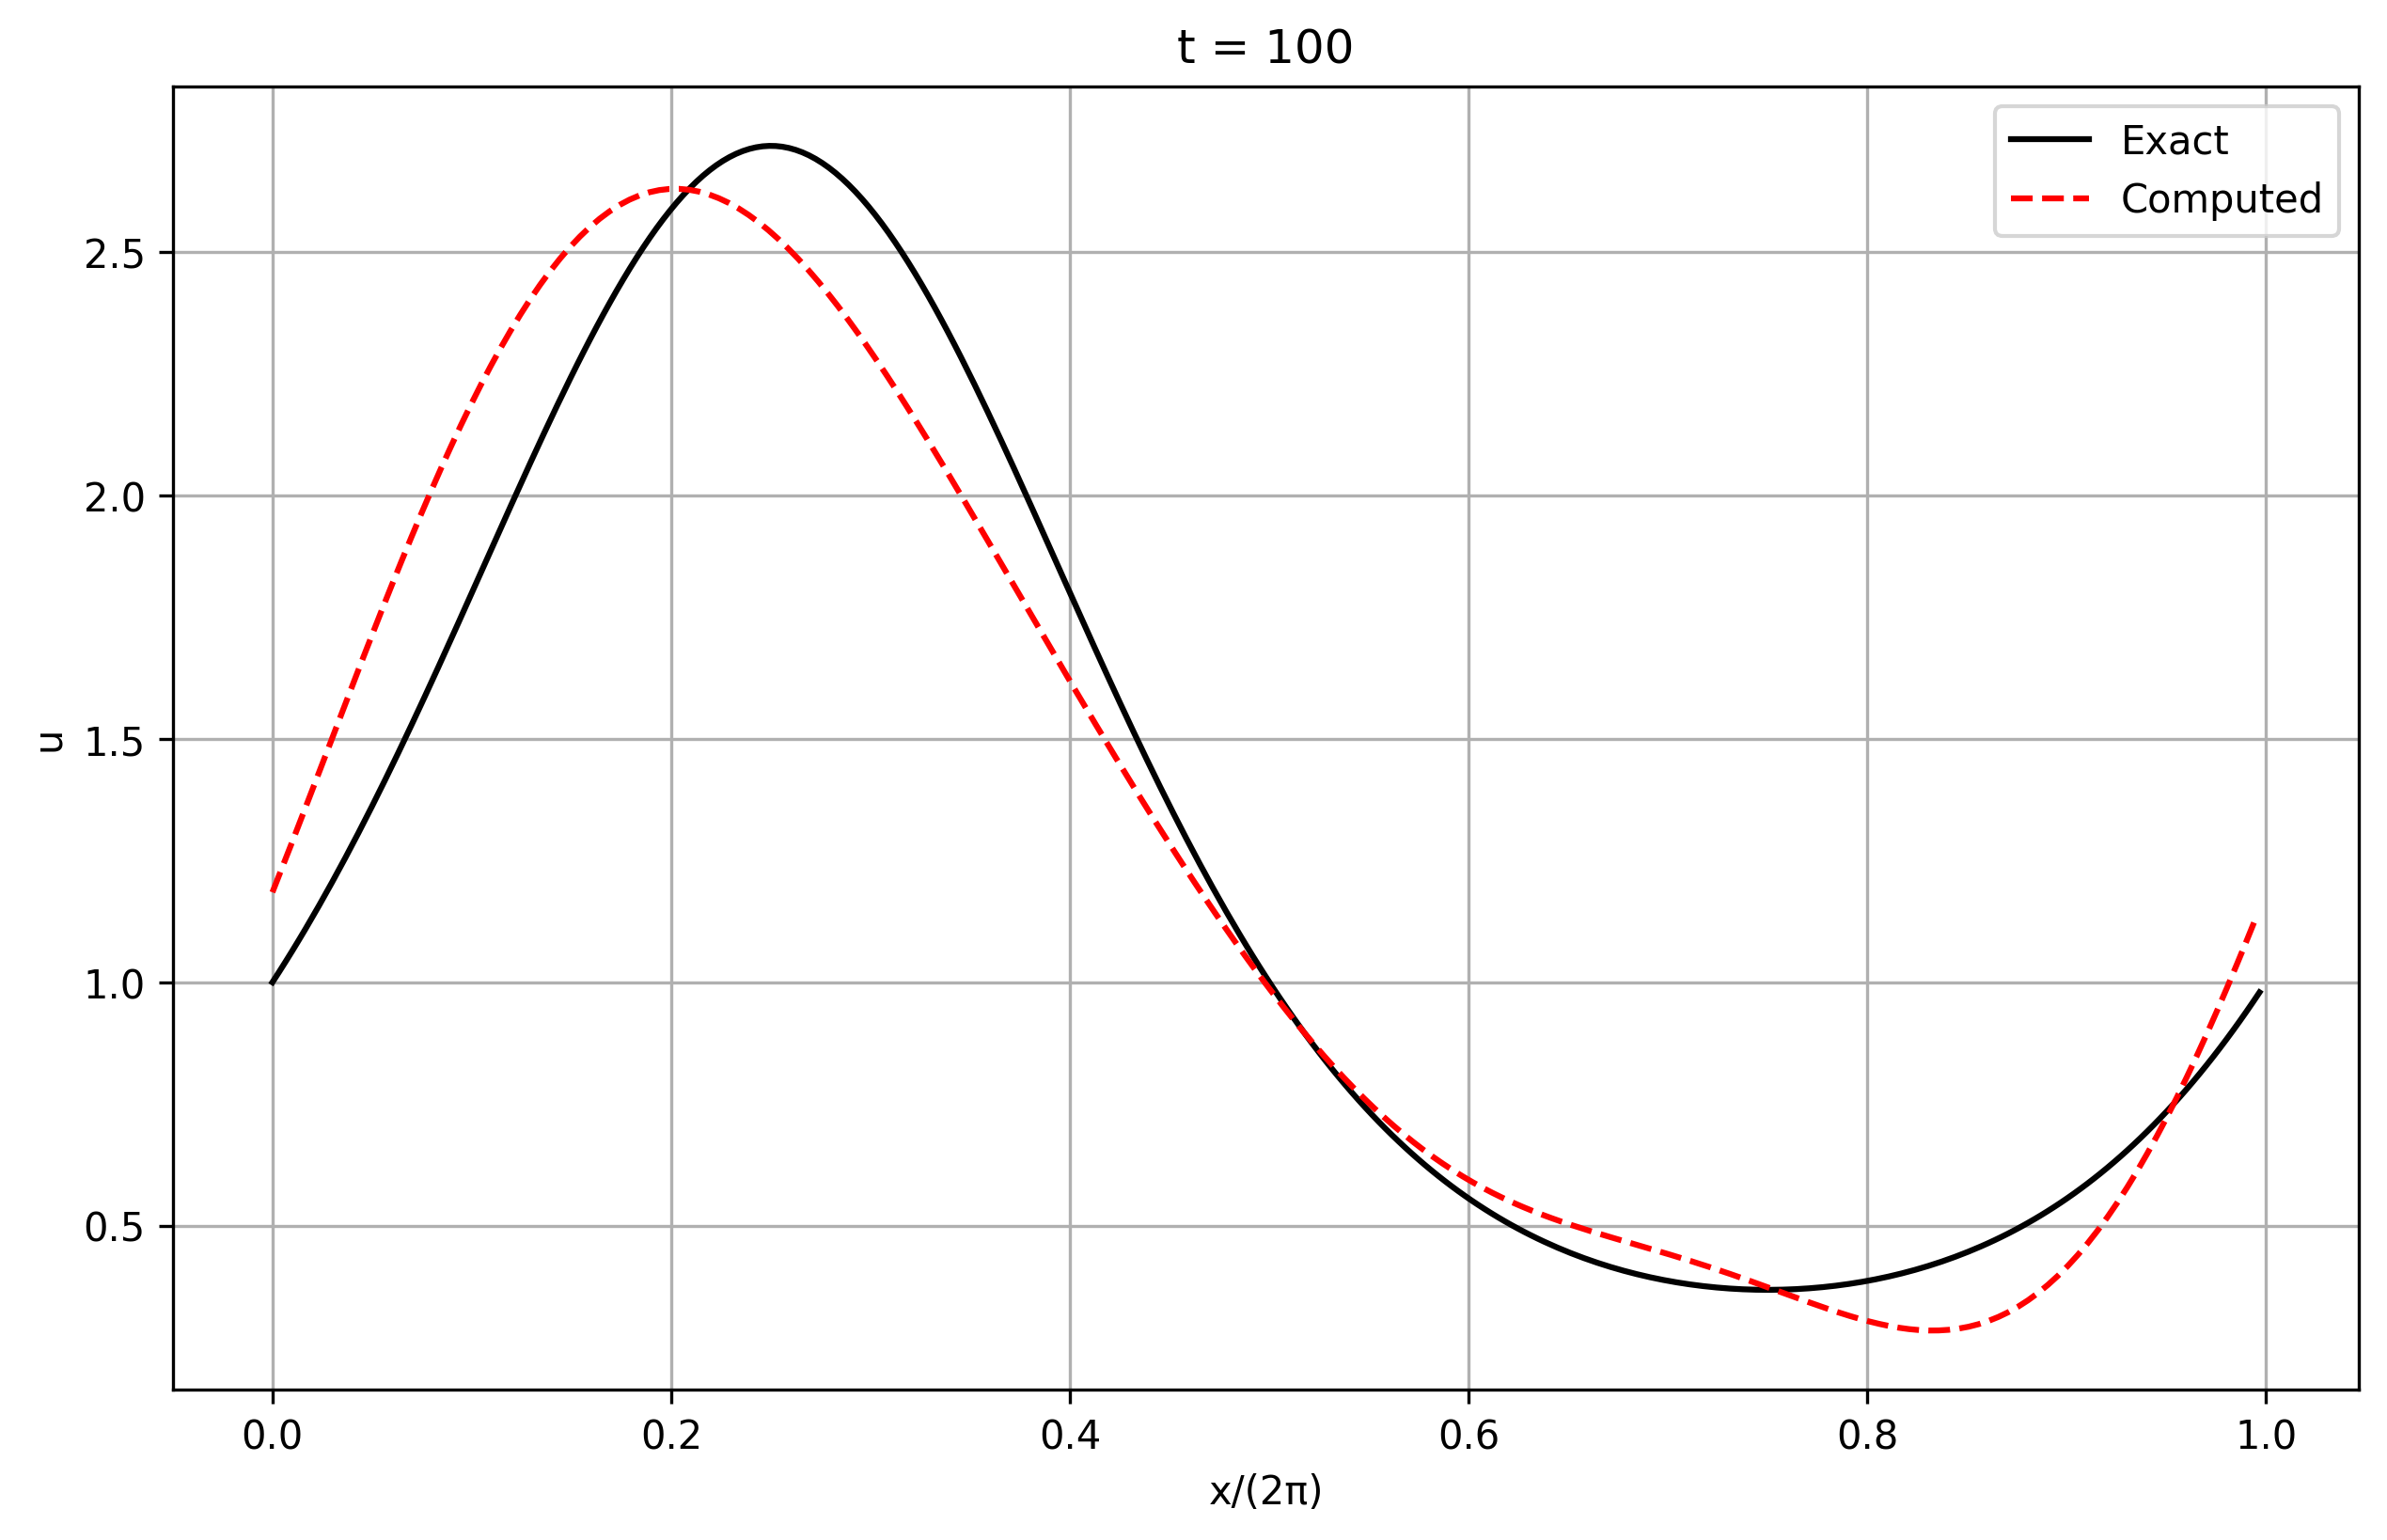
\includegraphics[width=\textwidth]{figures/long_time_second_order_100.png}
        \caption{t = 100}
    \end{subfigure}
    \begin{subfigure}[b]{0.32\textwidth}
        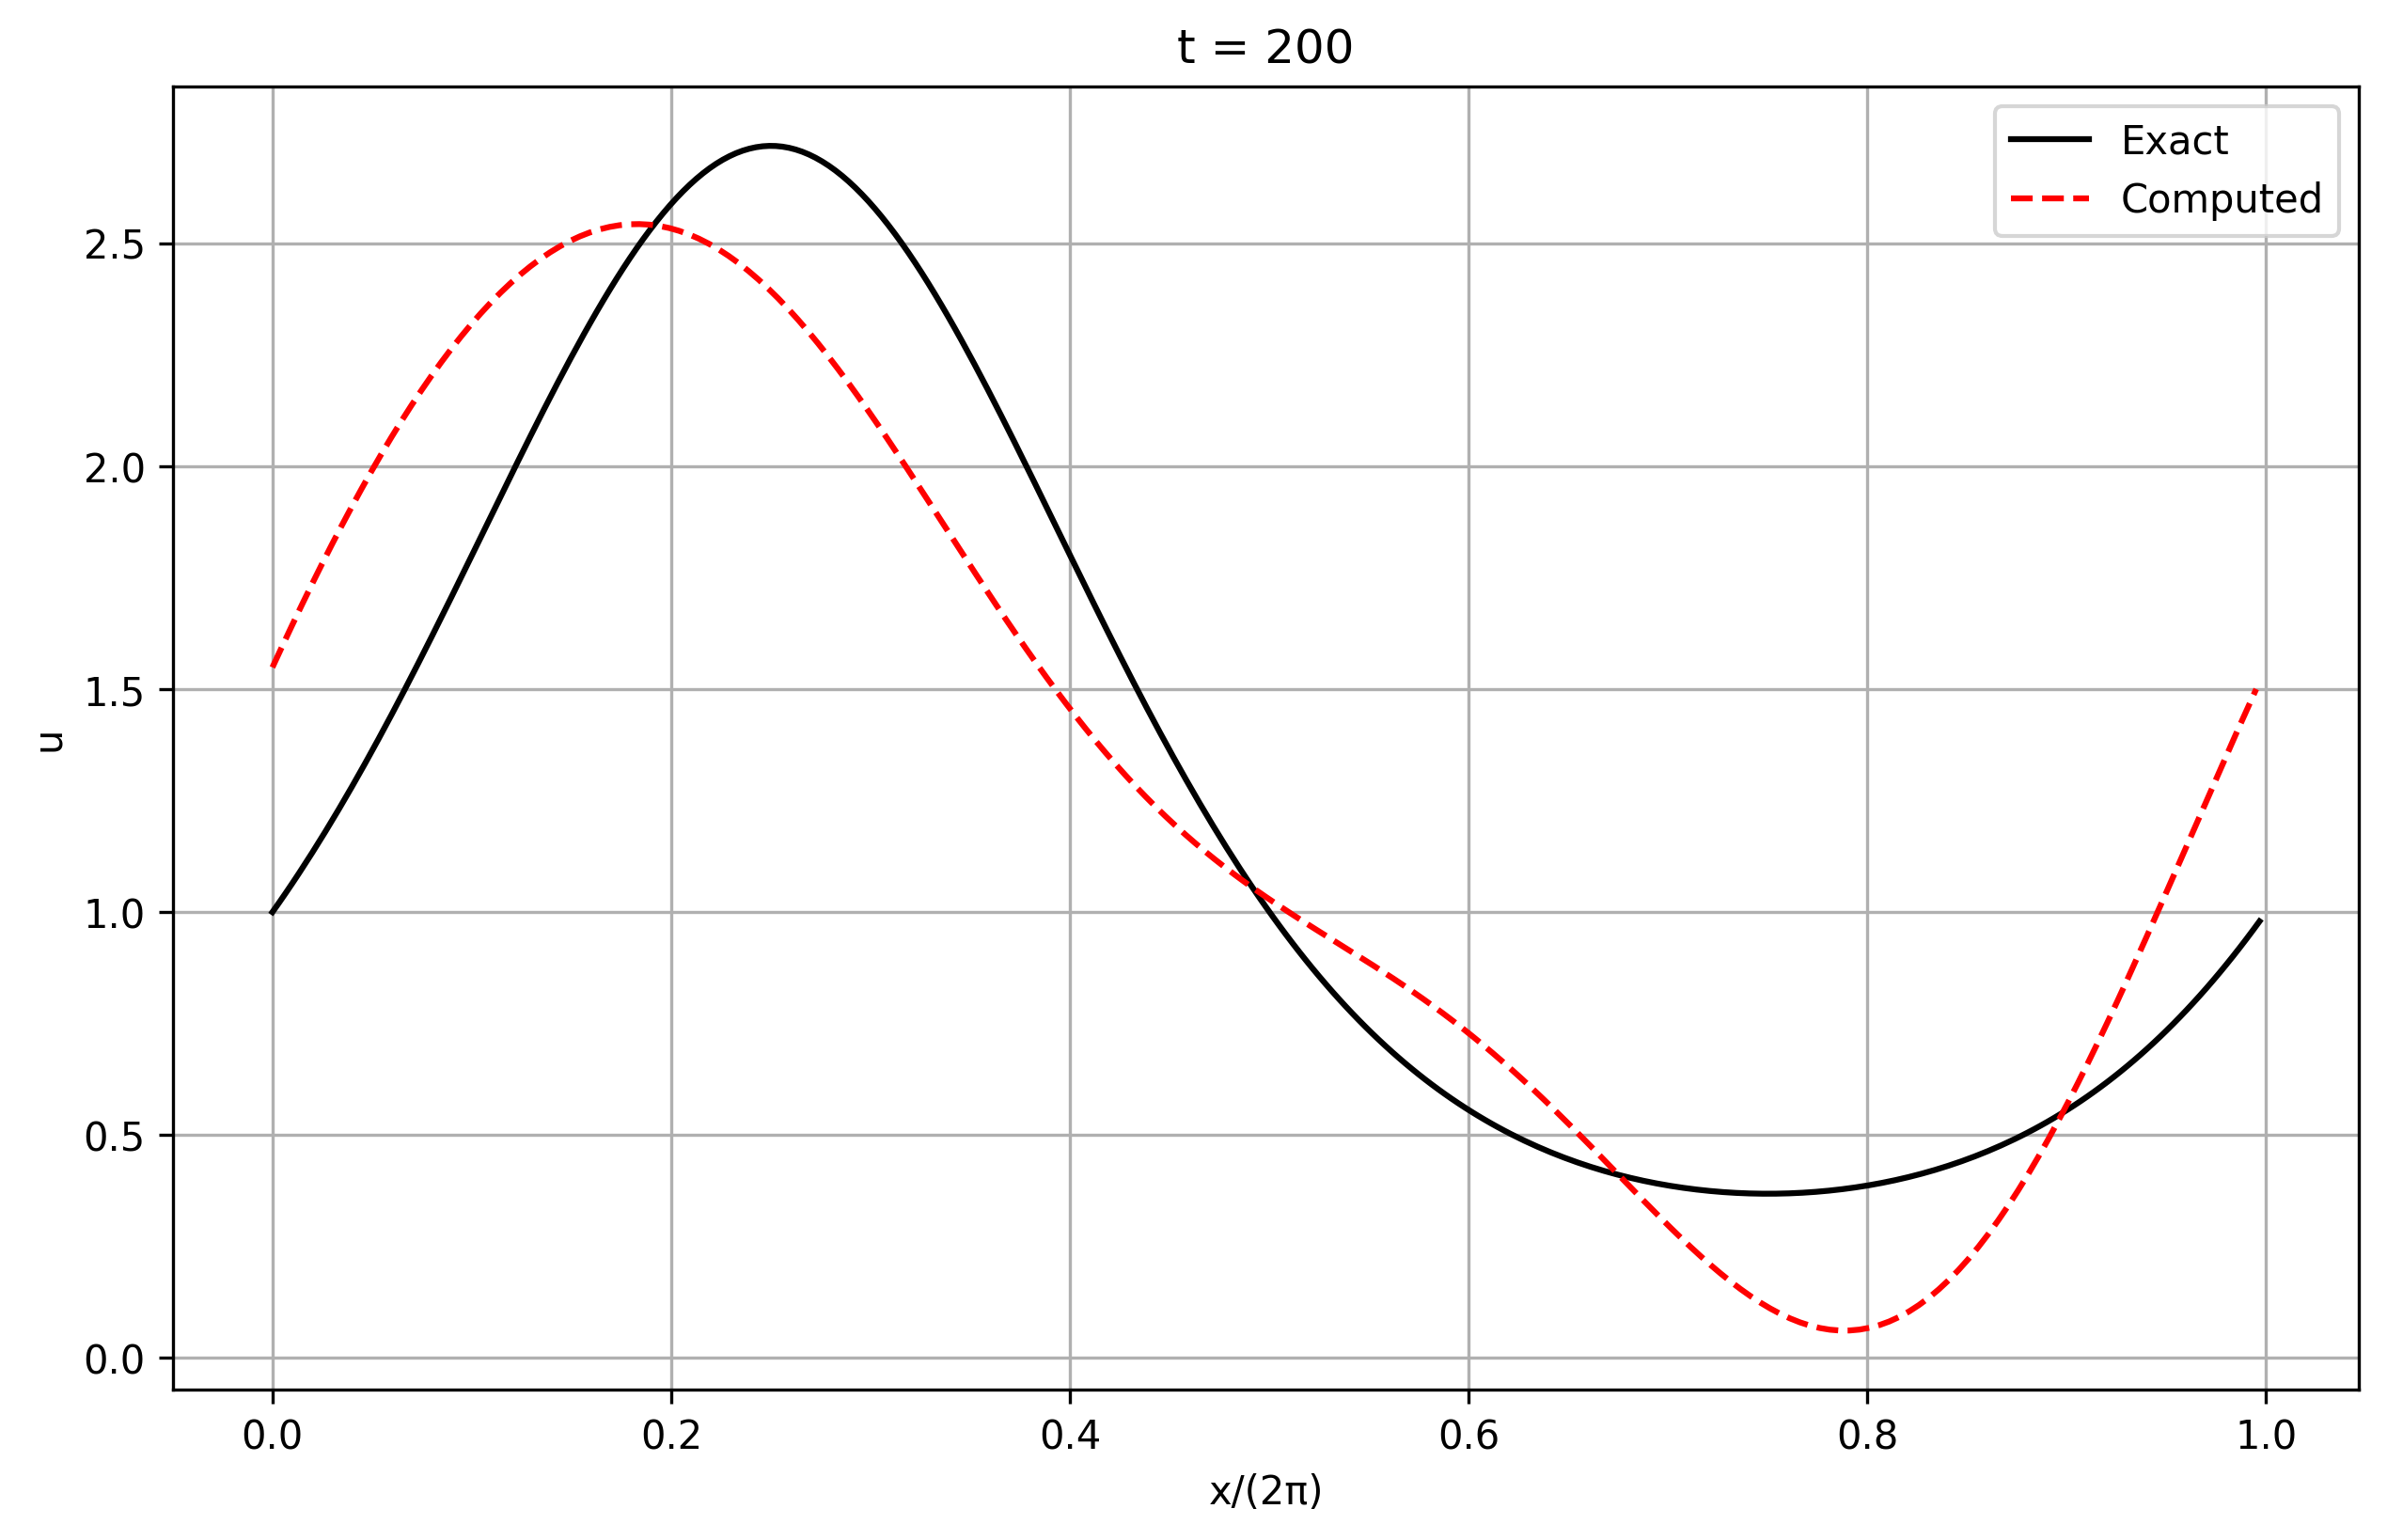
\includegraphics[width=\textwidth]{figures/long_time_second_order_200.png}
        \caption{t = 200}
    \end{subfigure}
    \caption{Long-time integration results for second order method (N=200)}
    \label{fig:long_time_second}
\end{figure}

The figures show that both methods maintain the solution profile well over the long integration period. The infinite order method achieves comparable accuracy to the second order method despite using only N=10 grid points, compared to N=200 for the second order method. This demonstrates the efficiency advantage of the infinite order method for this periodic problem.

\subsection{Conclusions}
The infinite order method demonstrates superior accuracy for small N, achieving near machine precision with just 32 grid points. The fourth-order method shows excellent convergence for smooth solutions, while the second-order method provides reliable but less accurate results. All methods maintain stability in long-time integration, with their accuracy consistent with their theoretical convergence rates.

\end{document}
